%!TEX program=xelatex
% PromptMatte 课程报告 —— 基于 CVPR 中文模板（cvpr.cls + ctex，xelatex 编译）
\documentclass[final]{cvpr}

\usepackage[UTF8]{ctex}
\usepackage{times}
\usepackage{epsfig}
\usepackage{graphicx}
\usepackage{amsmath}
\usepackage{amssymb}
\usepackage{bm}
\usepackage{booktabs}
\usepackage{subfigure}
\usepackage{multirow}

\usepackage{enumitem}
\setenumerate[1]{itemsep=0pt,partopsep=0pt,parsep=\parskip,topsep=5pt}
\setitemize[1]{itemsep=0pt,partopsep=0pt,parsep=\parskip,topsep=5pt}

\usepackage[breaklinks=true,colorlinks,bookmarks=false]{hyperref}

% [final] 类选项即终稿模式（显示作者、无审稿行号）
\def\cvprPaperID{0005}
\def\confYear{计算机视觉课程大作业 2026}
\def\httilde{\mbox{\tt\raisebox{-.5ex}{\symbol{126}}}}

\graphicspath{{figures/}}

\begin{document}

\renewcommand{\figref}[1]{图\ref{#1}}
\renewcommand{\tabref}[1]{表\ref{#1}}
\renewcommand{\equref}[1]{式\ref{#1}}
\renewcommand{\secref}[1]{第\ref{#1}节}

%%%%%%%%% TITLE
\title{PromptMatte：基于视觉基础模型融合的零训练精细抠图与换背景系统}

\author{梁景铭 \quad 史傅冠华 \quad 张竣翔 \\
南开大学 计算机学院 \quad 第五组 \\
{\tt\small 计算机视觉课程大作业}
}

\maketitle

%%%%%%%%% ABSTRACT
\begin{abstract}
精细抠图（image matting）需要在头发、毛发、玻璃等半透明边界上估计连续的透明度
$\alpha$，是背景替换、背景虚化与视频合成等编辑应用的核心。
传统方法依赖人工 trimap 或专门训练，复现成本高；而以 SAM 为代表的视觉基础模型
擅长目标定位，却只能输出粗糙的二值掩码，难以刻画精细边界。
本文提出 \textbf{PromptMatte}：一个\textbf{零训练（training-free）}的精细抠图与换背景系统，
它把开放词汇定位、精细 $\alpha$ 估计、视频时序稳定与背景编辑串成一条统一主线，
全程不更新任何模型权重，所有增益都来自\textbf{在推理阶段注入一致性先验}。
具体地，上游用 SAM2 配合 Prompt Ensemble 与 IoU 引导重排序得到稳定定位；
图像端在 ZIM 输出的软 $\alpha$ 上注入\textbf{翻转等变一致性先验}（PromptMatte-TTA-GF）
并以检测框作为\textbf{空间先验}（Box-Support Prior, BSP）抑制框外泄漏；
视频端复用图像主线的首帧 $\alpha$，并把同一条一致性先验从空间推广到时间，
形成\textbf{双向时序平滑}。
在 MicroMat-3K 的 valid706 官方提示子集上，本文方法在 SAD、MSE、MAE、Boundary~SAD
四项指标上全面优于 ZIM 官方 bbox 基线；在 20 段视频上，双向时序平滑是唯一能在
\textbf{几乎不损精度}的前提下提升时序一致性的策略。
\end{abstract}

%%%%%%%%% BODY
\section{引言}
\label{sec:intro}

图像与视频抠图的目标，是在复杂场景中分离目标前景，并在头发、毛发、玻璃等区域
估计出连续的软边界透明度 $\alpha\in[0,1]$，进而支持背景替换、背景虚化与海报合成等应用。
形式上，给定图像 $\mathcal{I}$ 与目标提示 $b$，抠图可写作
\begin{equation}
\mathrm{PromptMatte}(\mathcal{I}, b)\rightarrow \alpha^\star\in[0,1]^{H\times W},\quad
C=\alpha^\star F+(1-\alpha^\star)B,
\label{eq:matting}
\end{equation}
其中 $F$、$B$ 分别为前景与背景，$C$ 为合成结果。
抠图真正的难点不在于“把目标框出来”，而在于边界处的连续透明度估计——
发丝、毛发、半透明与细结构都不是非黑即白的硬边界。
该能力广泛支撑电商商品图、人像修图、短视频换背景与海报合成等场景，
并贯穿目标定位、精细抠图与结果合成三个环节，因而具有直接的实用价值。

\noindent\textbf{现有方法的局限。}
一方面，传统抠图往往依赖人工绘制的 trimap，或需要在抠图数据上专门训练，
复现成本高、难以规模化；另一方面，SAM~\cite{sam}、SAM2~\cite{sam2} 等视觉基础模型
虽然能准确定位目标，却只输出硬的二值掩码，在发丝、半透明边缘处只能硬切，
无法直接用于换背景。如何在\textbf{不训练}的前提下，把“准确的定位”与“精细的
$\alpha$”衔接起来，是本文要解决的核心问题。

\noindent\textbf{本文思路。}
我们不重新训练大模型，而是\textbf{复用现成的视觉基础模型}，把系统的全部创新放在
\textbf{推理阶段的先验注入}上。贯穿整个系统的，是一条简单而统一的\emph{一致性先验}：
一个正确的 $\alpha$，在变换下应当保持一致。该先验在图像上表现为\textbf{翻转等变}
（同一张图翻转后预测应与原图一致），在视频上自然推广为\textbf{时序一致}
（相邻帧的 $\alpha$ 应当一致）。正是这条先验，把图像分支与视频分支统一成同一套方法。

\noindent\textbf{贡献。}本文的主要贡献如下：
\begin{itemize}
\item 提出一个\textbf{零训练}的精细抠图与换背景系统 PromptMatte，将 SAM2 定位、
ZIM 精细抠图、视频时序稳定与背景编辑串成一条统一主线（\secref{sec:method}）。
\item 上游分割端，提出 \textbf{Prompt Ensemble + IoU 引导重排序}与多尺度推理，
显著提升 bbox 提示下的掩码稳定性（\secref{sec:upstream}）。
\item 图像抠图端，提出 \textbf{PromptMatte-TTA-GF}（翻转等变一致性 + 边缘感知投影）
与 \textbf{Box-Support Prior}，在 ZIM 输出之上以先验注入的方式细化边界，全程零训练
（\secref{sec:matting}）。
\item 视频端，复用图像首帧结果，并把一致性先验推广到时间维度，提出\textbf{双向时序平滑}
（\secref{sec:video}）。
\item 在 MicroMat-3K valid706 与 20 段视频上验证，本文方法在多项指标上全面优于基线
（\secref{sec:exp}）。
\end{itemize}

\begin{figure}[t]
\centering
\subfigure[输入图像]{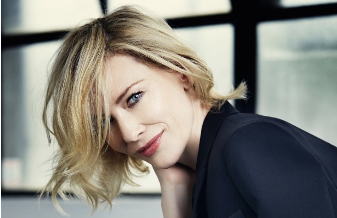
\includegraphics[width=0.235\linewidth]{teaser_input.png}}
\subfigure[SAM 粗分割]{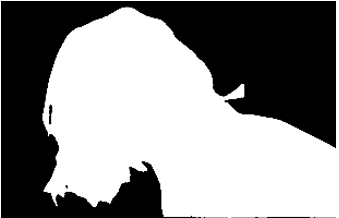
\includegraphics[width=0.235\linewidth]{teaser_sammask.png}}
\subfigure[精细 $\alpha$]{
\includegraphics[width=0.235\linewidth]{teaser_alpha.png}}
\subfigure[换背景结果]{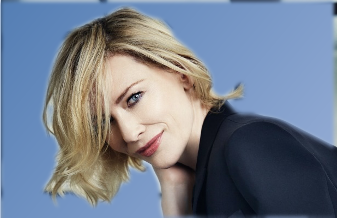
\includegraphics[width=0.235\linewidth]{teaser_composite.png}}
\caption{从粗分割到精细 $\alpha$ 再到换背景。SAM 只给出硬的二值掩码，
经本文方法细化为连续的软 $\alpha$ 后，即可干净地完成背景替换与虚化。}
\label{fig:teaser}
\end{figure}

\section{相关工作}
\label{sec:related}

\noindent\textbf{开放词汇分割与定位。}
SAM~\cite{sam} 提出可提示的分割范式，SAM2~\cite{sam2} 将其扩展到图像与视频并显著提速；
Grounded-SAM~\cite{groundedsam} 通过引入文本编码器实现开放词汇定位。
这些模型擅长回答“目标在哪里”，但输出为接近二值的掩码，并不直接给出软 $\alpha$。
SAM2 采用轻量高效的 Hiera 主干，原生支持 bbox 与 points 提示，并对每个提示输出
多候选掩码及其 IoU 置信度——后者恰好为下游的候选重排序提供了可靠信号。
本文以 SAM2 作为上游定位器，仅使用其 bbox 提示能力，不引入额外的文本分支。

\noindent\textbf{图像抠图。}
抠图的核心是求解欠定的合成方程~\equref{eq:matting}：每个像素仅观测到颜色 $C$，
却要同时反解 $F$、$B$、$\alpha$ 三个未知量。传统方法借助人工 trimap 把图像划分为
确定前景、确定背景与不确定边界带，从而把求解范围收缩到那条窄带上，但 trimap 的标注成本高、
难以规模化。Matting Anything~\cite{mam} 尝试在 SAM 基础上做抠图；
ZIM~\cite{zim} 面向零样本抠图，保留 SAM 式的点/框提示交互，但通过层次化像素解码器
输出连续 soft matte，且无需抠图标注即可训练。本文以 ZIM 作为精细抠图基座，
用 SAM2 自动产生的框提示替代人工 trimap，并在 ZIM 输出之上注入先验做细化。

\noindent\textbf{视频抠图与时序稳定。}
MatAnyone2~\cite{matanyone} 面向人像视频抠图，但逐帧推理会带来 $\alpha$ 抖动与边界闪烁。
本文不训练额外的时序模型，而是以一致性先验的形式做边界带时序平滑。

\noindent\textbf{测试时增强与引导滤波。}
测试时增强（TTA）通过对输入做变换并融合预测来降低方差；
引导滤波（Guided Filter）~\cite{gf} 是一种保边平滑算子，可用引导图的边缘结构约束输出。
本文将二者组合，作为翻转等变一致性先验的具体实现。

\section{方法}
\label{sec:method}

\subsection{系统总览}
\label{sec:overview}
PromptMatte 是一条从定位到合成的统一主线，包含图像与视频两条分支，全程不训练。

\noindent\textbf{图像主线。}给定图像与 official bbox：SAM2 给出若干候选掩码，
经 Prompt Ensemble 与 IoU 引导重排序选出最优者、再以 Guided Filter 修边，得到稳定的粗定位；
随后交给 ZIM 得到连续的软 $\alpha$；在 ZIM 输出之上依次注入 \textbf{TTA-GF} 与 \textbf{BSP}
两个先验做精细化；最后通过 Composer 输出 RGBA、背景替换或背景虚化。

\noindent\textbf{视频分支。}视频不从零开始，而是\textbf{复用}图像主线算出的首帧 $\alpha$
作为种子，交给 MatAnyone2 得到逐帧 $\alpha$，再施加\textbf{双向时序平滑}稳定边界，完成视频换背景。

\noindent 综上，图像主线可概括为如下流水线，前一步的输出即后一步的输入：
\begin{enumerate}[label=(\arabic*)]
\item 输入图像 $+$ official bbox；
\item SAM2 输出候选掩码；
\item Prompt Ensemble $+$ IoU 引导重排序选出最优候选；
\item Guided Filter 修边，得到稳定的粗定位；
\item ZIM 估计连续软 $\alpha$；
\item PromptMatte-TTA-GF（翻转等变一致性 $+$ 边缘投影）细化边界；
\item Box-Support Prior 抑制框外泄漏；
\item Composer 输出 RGBA、背景替换或虚化。
\end{enumerate}
视频分支在第 (5)\,$\sim$\,(6) 步得到的首帧结果之上，接 MatAnyone2 与双向时序平滑。

\noindent\textbf{统一的一致性先验。}贯穿全系统、也是核心创新的，是一致性先验的复用：
它在图像上是 TTA-GF（空间维度的翻转等变），在视频上是双向时序平滑（时间维度的相邻帧一致）。
同一条先验落在空间与时间，把图像与视频接成同一套方法，而非彼此独立的模块。

值得强调的是，本文的全部增益都不来自训练，而来自“在恰当的位置注入恰当的先验”：
我们不改动任何基础模型的权重，而是把领域知识（变换一致性、目标必在框内、相邻帧连续）
显式地写进推理过程。这一设计带来三点好处：一是\textbf{可复现性强}，无需 GPU 重新训练即可复刻；
二是\textbf{模块解耦}，上游定位、抠图基座可随基础模型升级而平滑替换；
三是\textbf{可解释}，每一步增益都能归因到一条明确的先验，而非黑盒拟合。

\subsection{上游开放词汇分割}
\label{sec:upstream}
该模块回答“目标在哪里”，为下游抠图提供稳定的 bbox/points 入口与候选掩码。

\noindent\textbf{模型选型。}我们选用 SAM2.1 Hiera-Base+（约 80.8M 参数）：其 Hiera 架构
轻量高效、原生支持 bbox 与 points 提示、并输出多候选掩码与 IoU 置信度，便于做重排序；
相较 SAM3 推理更快、相较 Grounded-SAM-2 无需额外文本编码器，显存开销更小。
全过程保持 zero-training。

\noindent\textbf{Prompt Ensemble 与 IoU 引导重排序。}
SAM2 的单次 bbox 推理易受局部纹理干扰而选到次优掩码。我们用多组提示策略
（如 \emph{bbox-only} 与 \emph{bbox + 正点}）生成候选掩码，再用一个综合打分挑选最优：
\begin{equation}
S(m)=0.55\cdot\mathrm{IoU}(m)+0.25\cdot\mathrm{conn}(m)+0.20\cdot\mathrm{bbox\_cov}(m),
\label{eq:rerank}
\end{equation}
其中 IoU 为 SAM2 自身的掩码质量置信度（最可靠信号），$\mathrm{conn}$ 由连通分量数衡量
掩码碎片化程度（惩罚零散碎片），$\mathrm{bbox\_cov}$ 约束掩码对检测框的合理覆盖。

\noindent\textbf{多尺度推理。}单尺度推理对分辨率敏感。我们在 $\{0.75\times,1.0\times,1.25\times\}$
三个尺度分别运行 SAM2，将掩码 resize 回原分辨率后平均，稀释单尺度的随机边界偏差，
其代价是约三倍推理时间。该模块作为可选项与 ensemble 叠加：
我们先在每个尺度内部各自做 ensemble 重排序，再跨尺度平均，使“选最优候选”与
“抑制单尺度偏差”两种机制互补叠加。需要说明的是，最终提交方法（ensemble\_guided）
出于精度与开销的平衡并未启用多尺度，相关取舍见 \secref{sec:exp-sam} 的消融。

\subsection{精细抠图：从二值掩码到软 \texorpdfstring{$\alpha$}{alpha}}
\label{sec:matting}
该模块回答“边界够不够精细”，是本文的方法核心。

\noindent\textbf{ZIM 基座。}
ZIM~\cite{zim} 沿用 SAM 式提示架构：图像编码器与提示编码器分别提取图像特征与框/点提示，
解码器借掩码注意力聚焦目标，最后由层次化像素解码器逐级上采样、融合多尺度特征，
输出每个像素 $0\!\sim\!1$ 的连续 $\alpha$（\figref{fig:zim}）。
我们把 ZIM 当作\textbf{冻结的黑盒}使用——给框、出 $\alpha$，所有优化都作用在它的 soft matte 输出之上。

\begin{figure}[t]
\centering
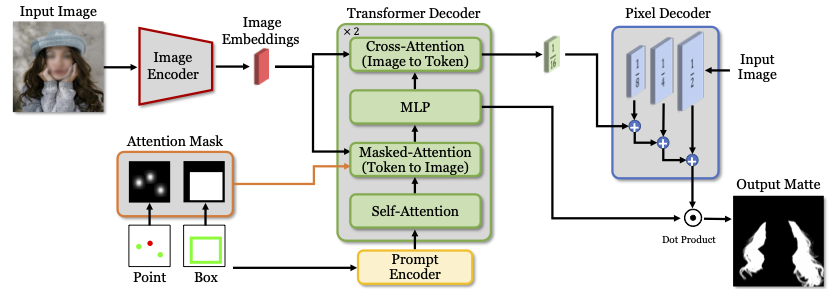
\includegraphics[width=0.96\linewidth]{zim_overview.png}
\caption{ZIM 原理示意。输入图像与提示，经图像/提示编码器与解码器，
最终由像素解码器输出连续 soft matte。图源：ZIM 官方项目~\cite{zim}。}
\label{fig:zim}
\end{figure}

\noindent\textbf{优化一：PromptMatte-TTA-GF。}
ZIM 的单次预测在边界处对视角方向与局部纹理较为敏感，同一目标换一个朝向，
边界就会产生偏差。我们将其建模为\textbf{翻转等变一致性}先验：理想情况下
$f_\theta\big(F(\mathcal{I})\big)$ 应与 $F\big(f_\theta(\mathcal{I})\big)$ 一致（$F$ 为水平翻转）。
据此，我们对原图与其翻转各预测一次、对齐后取平均，以抵消方向带来的随机误差；
再以原图 RGB 边缘作引导，用 Guided Filter~\cite{gf} 将 $\alpha$ 对齐到真实图像边缘：
\begin{align}
\alpha_0 &= f_\theta(\mathcal{I},b), \quad
\alpha_1 = F^{-1}\!\big(f_\theta(F(\mathcal{I}),F(b))\big),\\
\alpha_T &= \tfrac{1}{2}(\alpha_0+\alpha_1), \quad
\alpha_G = \mathrm{GF}(\mathcal{I},\alpha_T).
\label{eq:ttagf}
\end{align}
全过程不训练、不修改 ZIM 任何权重，仅在推理阶段注入这一先验，即可使边界更准、更稳。
直观上，原图与翻转图的两次预测对“朝向”这一干扰因素是\emph{独立}的，
其方向相关的随机误差在对齐平均后相互抵消，类似集成学习中的方差缩减；
而 Guided Filter 则把平滑后的 $\alpha_T$ 重新对齐到原图真实的颜色边缘上，
使发丝、硬边等结构既不被抹糊、也不发生偏移。

\noindent\textbf{优化二：Box-Support Prior（BSP）。}
在 TTA-GF 之后，仍有少数样本会在 official bbox 之外残留少量 $\alpha$。
注意到“目标必在框内”是一条可靠的\textbf{空间先验}，我们以检测框构造软支持图 $G$
（框内为 1、框外渐变为一个保守下限 $\eta$），并对 $\alpha_G$ 做温和的空间重加权：
\begin{equation}
G(x)=S(x)+\big(1-S(x)\big)\eta,\quad
\alpha_B(x)=\alpha_G(x)\big(1-\lambda+\lambda\,G(x)\big).
\label{eq:bsp}
\end{equation}
框内（$G\!\approx\!1$）保持不变，框外（$G\!\approx\!0$）按系数 $(1-\lambda)$ 压低。
为避免误伤贴近框边的合法前景，支持图在构造时对框做了轻微外扩与边缘模糊。
BSP 是一项保守的稳定化处理（\figref{fig:bsp}），几乎不影响主体，却能进一步清除框外泄漏与毛刺。
两个先验各司其职：TTA-GF 约束边界的对齐，BSP 约束前景的空间范围，二者互补。

\begin{figure}[t]
\centering
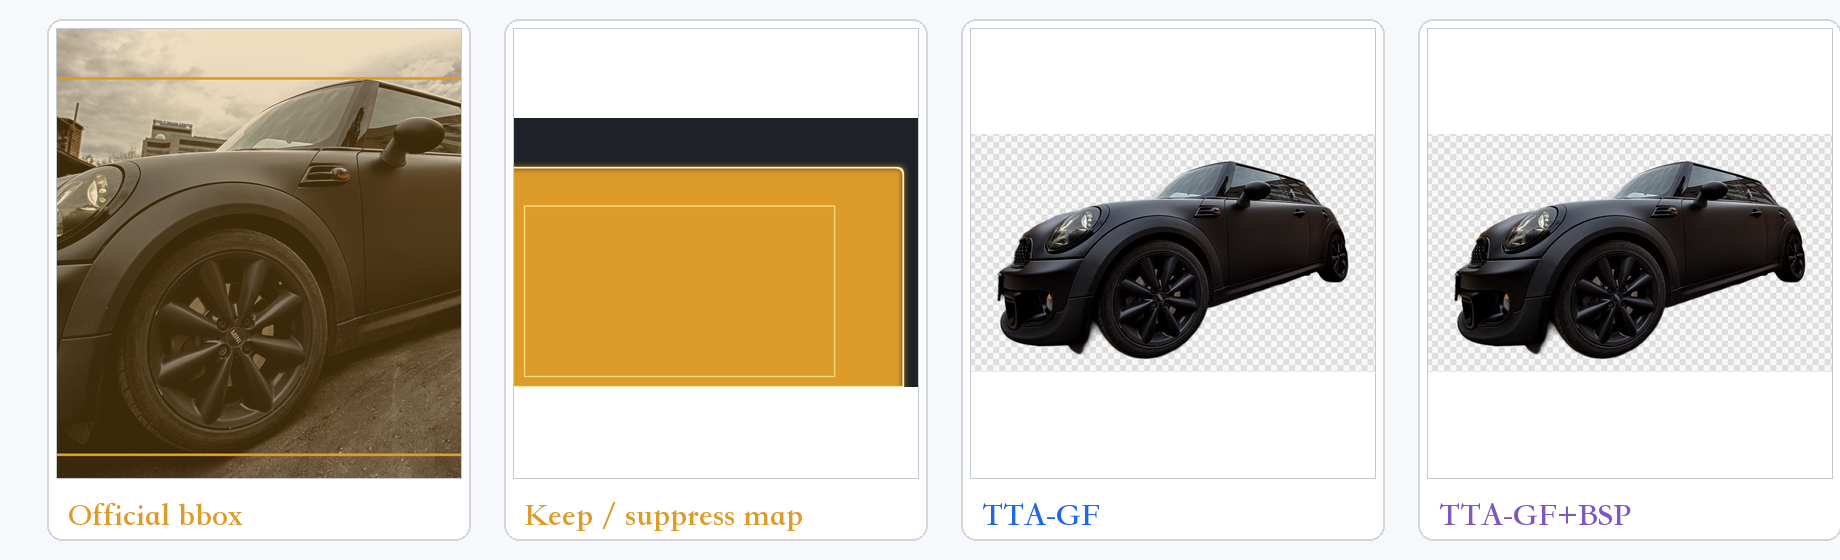
\includegraphics[width=0.98\linewidth]{bsp_cards.png}
\caption{Box-Support Prior：以检测框作为空间先验，框内保留、框外温和抑制，
进一步清除框外的 $\alpha$ 泄漏。}
\label{fig:bsp}
\end{figure}

\subsection{视频时序平滑}
\label{sec:video}
该模块回答“能否稳定地落地演示”。我们以 MatAnyone2~\cite{matanyone} 为视频基线，
但其逐帧推理会带来 $\alpha$ 抖动与边界闪烁，直接换背景会放大这种不稳定。

\noindent\textbf{首帧复用。}视频分支不另起炉灶，而是直接复用图像主线算出的首帧 $\alpha$
作为种子，相当于把图像端的全部精细化结果带入视频。

\noindent\textbf{双向时序平滑。}我们把图像端的一致性先验从空间推广到时间：
相邻帧的 $\alpha$ 应当一致。据此施加\textbf{双向}（同时利用过去帧与未来帧）时序平滑，
且\textbf{仅在边界带}（$\alpha\in[0.05,0.95]$）上作用，从而保护前景核区与发丝细节、避免过度模糊。
该模块同样复用邻帧信息而非训练时序模型——它不是事后的修补，而是同一条一致性先验在时间维度的落地。

\subsection{复杂度与部署}
\label{sec:complexity}
PromptMatte 的额外开销集中在推理阶段，且大多来自可裁剪的可选模块。
上游 SAM2.1 Hiera-Base+ 在 A10 上约 $1.16$ it/s（bbox-only）；
Prompt Ensemble 因生成多组候选而近似线性地增加前向次数，多尺度推理带来约三倍开销，二者均为可选项。
图像抠图端，翻转 TTA 使 ZIM 的前向次数翻倍，而 Guided Filter 与 BSP 都是轻量的逐像素后处理，开销可忽略；
视频端的双向时序平滑是一维时序滤波，复杂度与帧数线性相关。
由于全程不训练，整套系统无需 GPU 训练资源即可复现；
在对延迟敏感的部署中，可按精度/速度需求关闭 ensemble 与多尺度等可选模块，
仅保留 “ZIM\,$+$\,TTA-GF\,$+$\,BSP” 的核心链路。

\section{实验}
\label{sec:exp}

\subsection{实验设置}
\label{sec:setup}
\noindent\textbf{数据集。}图像端使用 MicroMat-3K 验证集中带 official bbox 提示的 valid706 子集
（706 张图像，每张配官方 bbox/points 与高质量 GT $\alpha$）。
视频端使用 YouTubeMatte 与 VideoMatt 各 10 段、共 20 段测试视频。

\noindent\textbf{指标。}图像端报告 SAD、MSE、$\mathrm{MAE}\times1000$ 与 Boundary~SAD（5px 边界带），
四项均\emph{越低越好}；视频端报告时序一致性 TC（越高越好）以及 SAD/MSE 的变化。
记预测与真值 $\alpha$ 分别为 $\hat\alpha$、$\alpha^*$。SAD 为绝对误差之和
$\sum_{x}|\hat\alpha(x)-\alpha^*(x)|$（按抠图惯例以 $/1000$ 计，故本文表中数值为个位数量级）；
MSE 为均方误差，MAE 为平均绝对误差（报告时 $\times1000$）；
Boundary SAD 仅在 GT 边界附近 5px 带内统计 SAD，专门刻画边缘质量；
TC 衡量相邻帧 $\alpha$ 的时序稳定程度，本文报告其相对基线的提升百分比。
所有方法在统一脚本下评分，Composer 应用不计入指标。
为保证公平，基线与各优化方法均使用\textbf{同一 official bbox} 推理、并用同一脚本统一评分；
valid706 强调“统一提示输入下的可复现对比”，而非追求论文级 SOTA。

\noindent\textbf{实现。}上游为 SAM2.1 Hiera-Base+；抠图基座为 ZIM ViT-B，
Guided Filter 半径取 1；视频双向平滑取 $\alpha=0.7$。全程无任何训练。

\subsection{上游分割消融}
\label{sec:exp-sam}
\tabref{tab:sam} 在 valid706 上以控制变量法逐项检验上游各模块。
以 bbox-only 单次推理 + 硬二值化为基线（bbox\_binary），逐步叠加 guided filter、
多尺度与 ensemble 重排序。可以看到：\emph{ensemble 重排序}是单点收益最大的模块
（SAD 相对基线下降约 11.5\%）；guided filter 显著改善边界（Boundary SAD $1.432\!\to\!1.271$）；
多尺度单独增益有限；三者协同的 \emph{ensemble\_guided} 取得最优，SAD、MAE、Boundary
相对基线分别改善约 $16.3\%$、$14.6\%$、$15.1\%$。

\begin{table}[t]
\centering
\small
\setlength{\tabcolsep}{3pt}
\begin{tabular}{lrrrr}
\toprule
方法 & SAD$\downarrow$ & MSE$\downarrow$ & MAE$\times$1k$\downarrow$ & Bnd-SAD$\downarrow$ \\
\midrule
\textbf{ensemble\_guided} & \textbf{2.774} & \textbf{0.000747} & \textbf{0.981} & \textbf{1.216} \\
ensemble\_multiscale\_guided & 2.915 & 0.000742 & 1.033 & 1.189 \\
ensemble\_rerank & 2.931 & 0.000843 & 1.037 & 1.380 \\
ensemble\_multiscale & 2.997 & 0.000796 & 1.062 & 1.279 \\
multiscale\_guided & 3.145 & 0.000828 & 1.089 & 1.249 \\
guided & 3.162 & 0.000845 & 1.095 & 1.271 \\
multiscale & 3.228 & 0.000894 & 1.119 & 1.341 \\
bbox\_binary (基线) & 3.314 & 0.000956 & 1.149 & 1.432 \\
\bottomrule
\end{tabular}
\caption{上游分割在 valid706 上的消融。最终采用 ensemble\_guided。}
\label{tab:sam}
\end{table}

\figref{fig:sam} 给出三个定性案例：大型目标（汽车）、小型目标与细结构物体。
按单图 SAD（同样以 $/1000$ 计）衡量，优化相对基线的改善十分显著：
大型目标 $13.559\!\to\!9.010$（$\downarrow33.5\%$），小型目标 $3.843\!\to\!0.348$（$\downarrow90.9\%$），
细结构物体 $2.562\!\to\!0.374$（$\downarrow85.4\%$）。
优化后掩码外溢更少、碎片显著减少、细边缘更清晰；尤其在小目标上，
基线常因局部纹理误选到次优候选导致掩码几乎全错，而 ensemble 重排序借助
\equref{eq:rerank} 的综合打分有效纠正了候选选择错误。

\noindent\textbf{消融归因。}三个模块的作用边界清晰：ensemble 重排序解决“选错候选”这类
\emph{离散}错误，单点收益最大；guided filter 解决“边界毛糙”这类\emph{连续}误差，
对 Boundary SAD 改善最明显（$1.432\!\to\!1.271$）；多尺度只平滑随机偏差，单独增益有限且开销大。
因此最终只保留 ensemble 与 guided 的组合，兼顾精度与效率。
\tabref{tab:samcase} 列出三个定性案例的单图 SAD 改善，可见在小目标与细结构上提升尤为巨大
（分别下降 $90.9\%$ 与 $85.4\%$），这正源于 ensemble 重排序对“候选选错”的纠正。

\begin{table}[t]
\centering
\small
\setlength{\tabcolsep}{8pt}
\begin{tabular}{lrrr}
\toprule
案例 & 基线 SAD & 优化 SAD & 改善 \\
\midrule
大型目标（汽车） & 13.559 & 9.010 & $-33.5\%$ \\
小型目标 & 3.843 & 0.348 & $-90.9\%$ \\
细结构物体 & 2.562 & 0.374 & $-85.4\%$ \\
\bottomrule
\end{tabular}
\caption{上游分割三个定性案例的单图 SAD（$/1000$）：优化相对基线改善显著。}
\label{tab:samcase}
\end{table}

\begin{figure}[t]
\centering
\subfigure[大型目标]{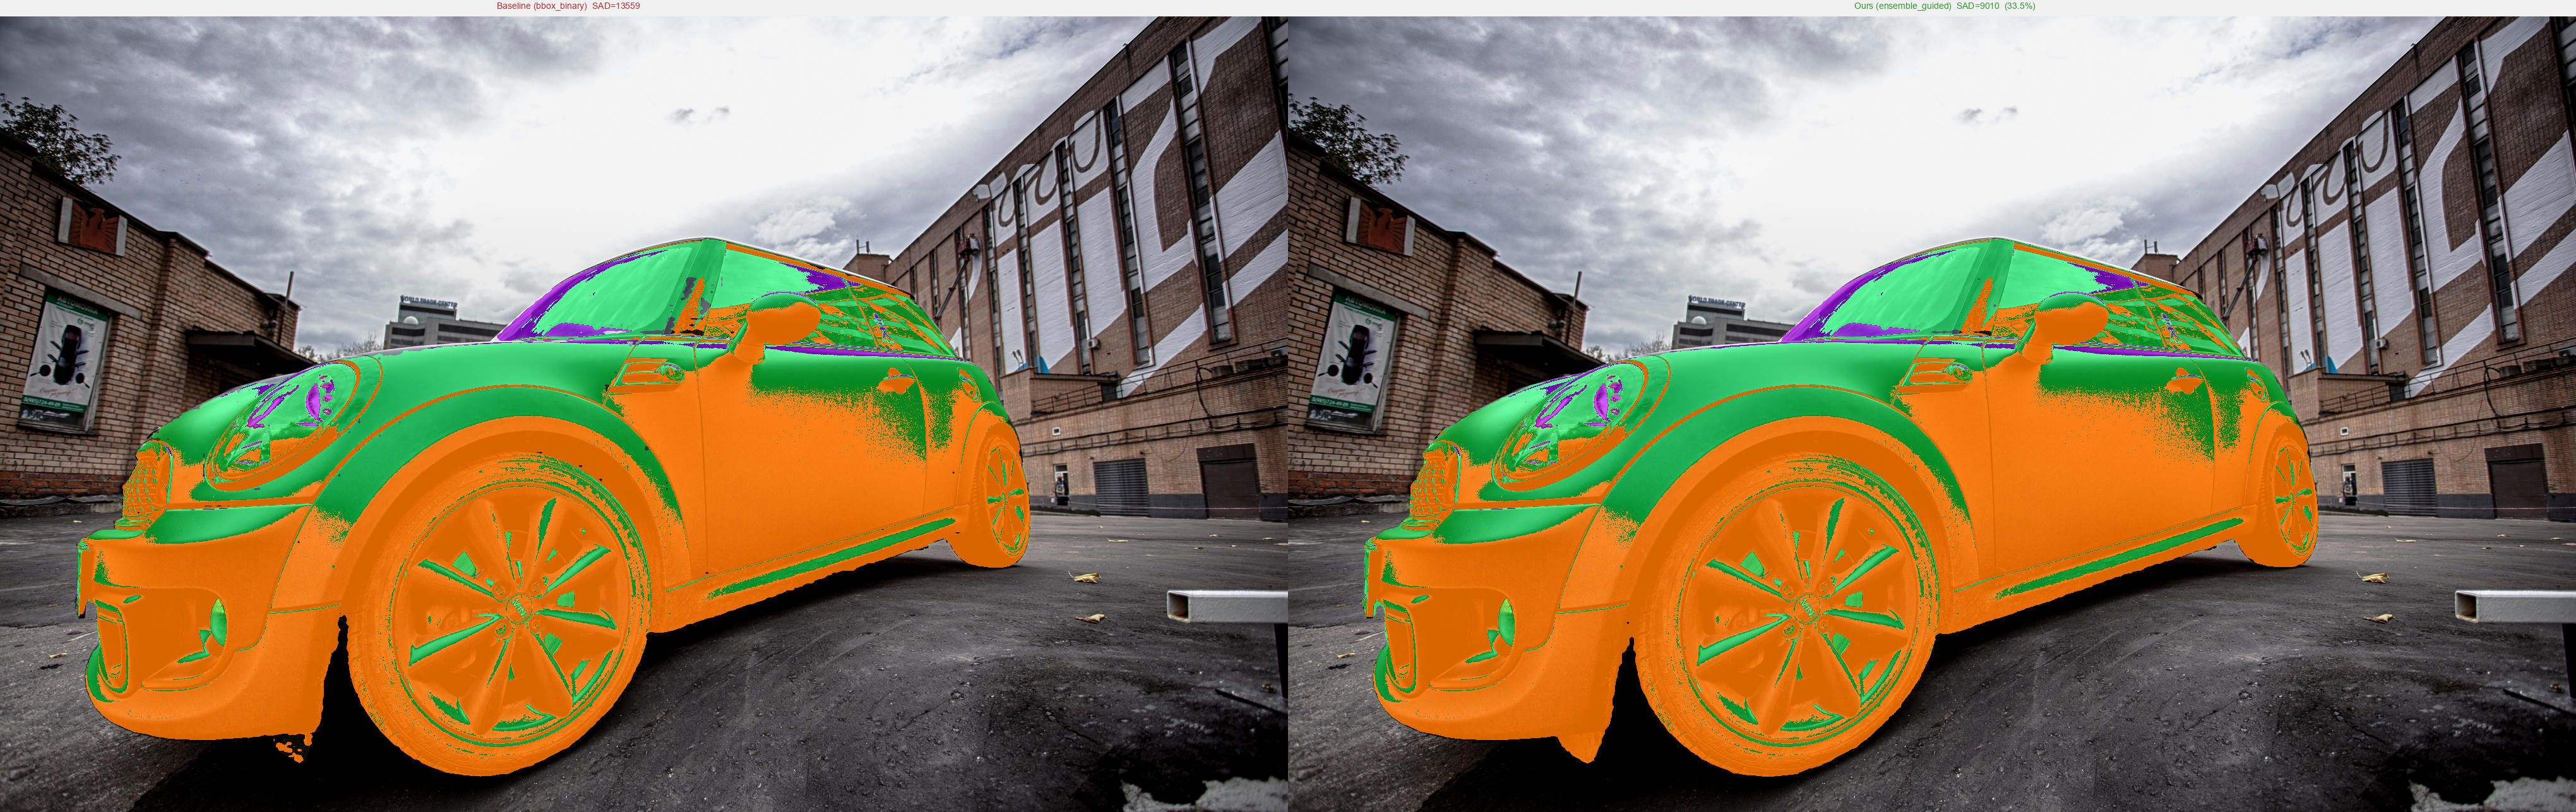
\includegraphics[width=0.32\linewidth]{sam_case1.png}}
\subfigure[小型目标]{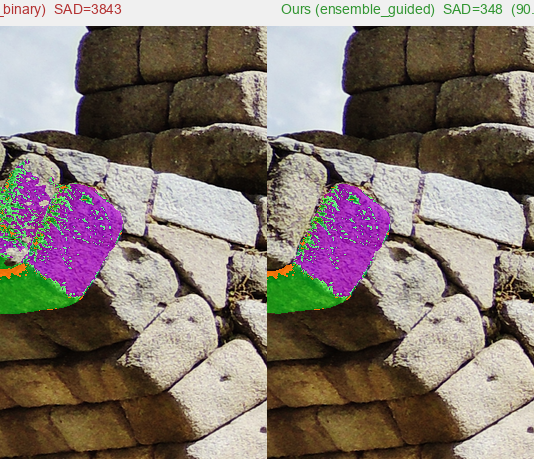
\includegraphics[width=0.32\linewidth]{sam_case2.png}}
\subfigure[细结构]{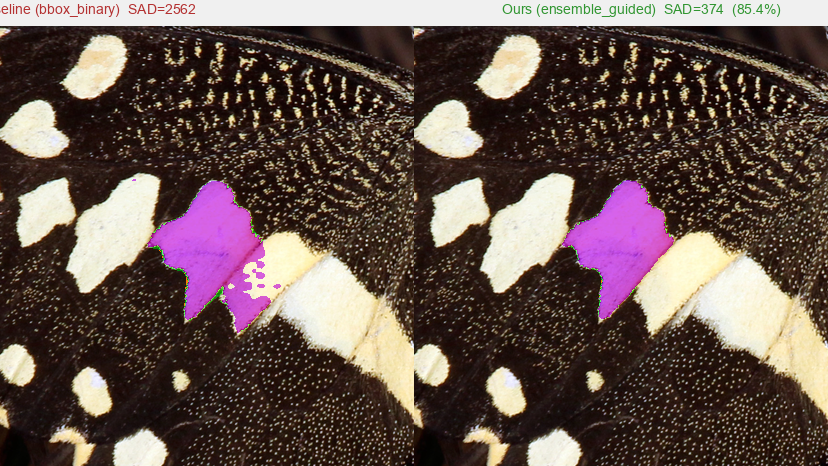
\includegraphics[width=0.32\linewidth]{sam_case3.png}}
\caption{上游分割定性对比：优化后（右）相比基线（左）边界更贴合、碎片更少。}
\label{fig:sam}
\end{figure}

\subsection{精细抠图主结果}
\label{sec:exp-zim}
\tabref{tab:zim} 在 valid706 上与 ZIM 官方 bbox 基线对比。
依次叠加 TTA-GF 与 BSP 后，四项指标逐步且全面下降：相对基线，
SAD 下降 $8.51\%$、MSE 下降 $23.14\%$、MAE 下降 $8.80\%$、Boundary SAD 下降 $13.35\%$，
其中 MSE 与边界误差改善最为显著。所有提升均在零训练前提下取得。

\begin{table}[t]
\centering
\small
\setlength{\tabcolsep}{3pt}
\begin{tabular}{lrrrr}
\toprule
方法 & SAD$\downarrow$ & MSE$\downarrow$ & MAE$\times$1k$\downarrow$ & Bnd-SAD$\downarrow$ \\
\midrule
ZIM bbox 基线 & 2.3201 & 0.0005795 & 0.8255 & 0.7366 \\
PromptMatte-TTA-GF & 2.1238 & 0.0004458 & 0.7533 & 0.6386 \\
\textbf{\;\;+ BSP（最终）} & \textbf{2.1227} & \textbf{0.0004454} & \textbf{0.7528} & \textbf{0.6383} \\
\midrule
相对基线改善 & $-8.51\%$ & $-23.14\%$ & $-8.80\%$ & $-13.35\%$ \\
\bottomrule
\end{tabular}
\caption{精细抠图在 valid706 上的主结果。本文方法四项全面优于 ZIM 基线。}
\label{tab:zim}
\end{table}

\figref{fig:zim_cases} 给出三个定性案例。约定红线为 ZIM 基线、绿线为 GT、蓝线为本文结果：
整车案例中 ZIM 在车轮附近外扩，本文结果更贴合车身；设备部件案例中 ZIM 边缘有毛刺与背景残留，
本文沿斜边更平直；热气球案例中 ZIM 边界偏移并带入背景，本文边缘更连续、更接近 GT。

\begin{figure*}[t]
\centering
\subfigure[整车目标]{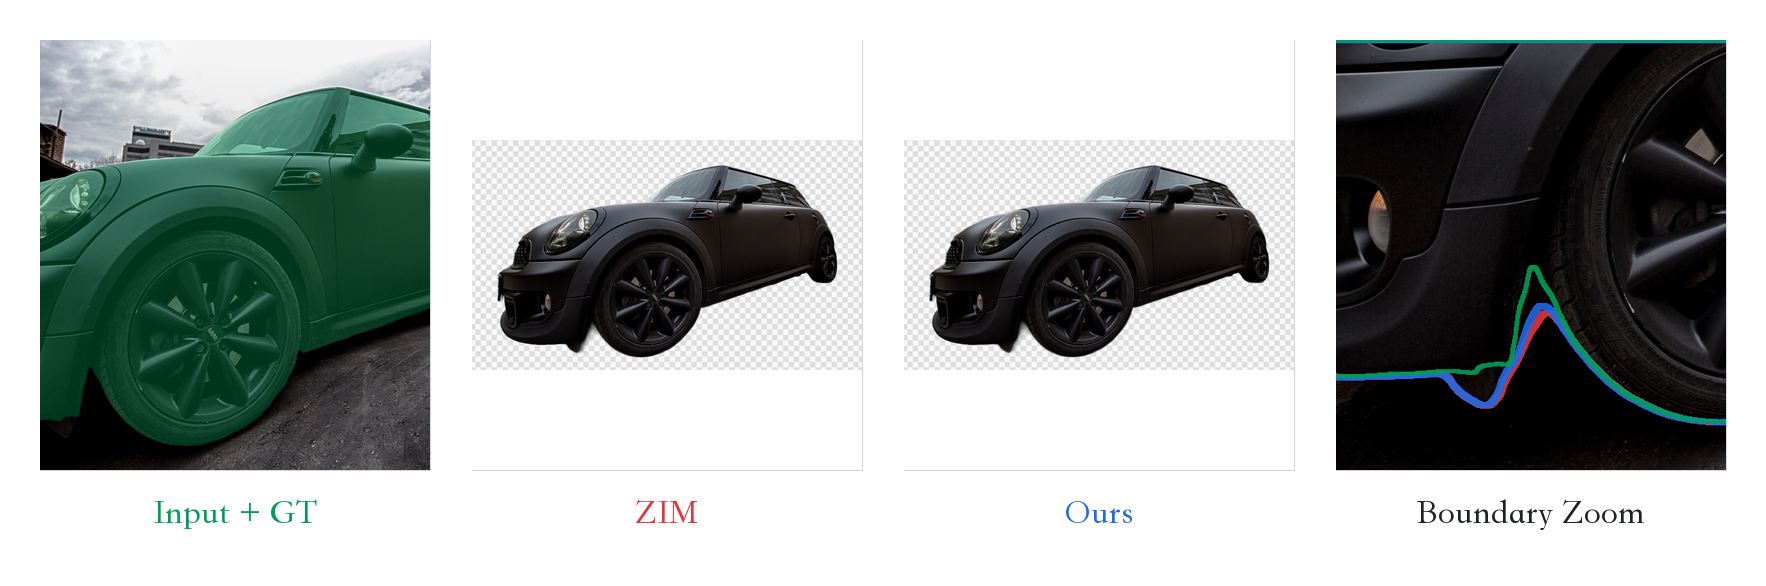
\includegraphics[width=0.32\linewidth]{zim_car.png}}
\subfigure[设备部件]{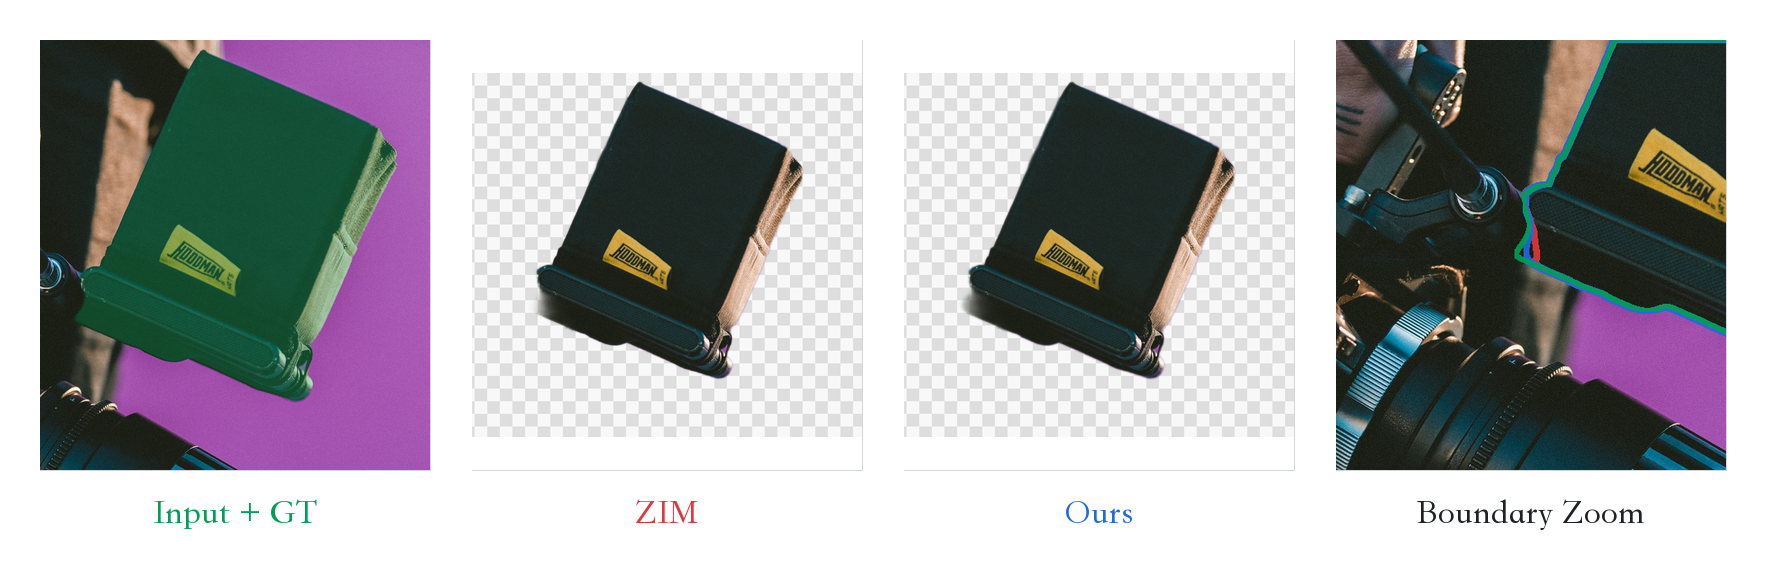
\includegraphics[width=0.32\linewidth]{zim_device.png}}
\subfigure[热气球]{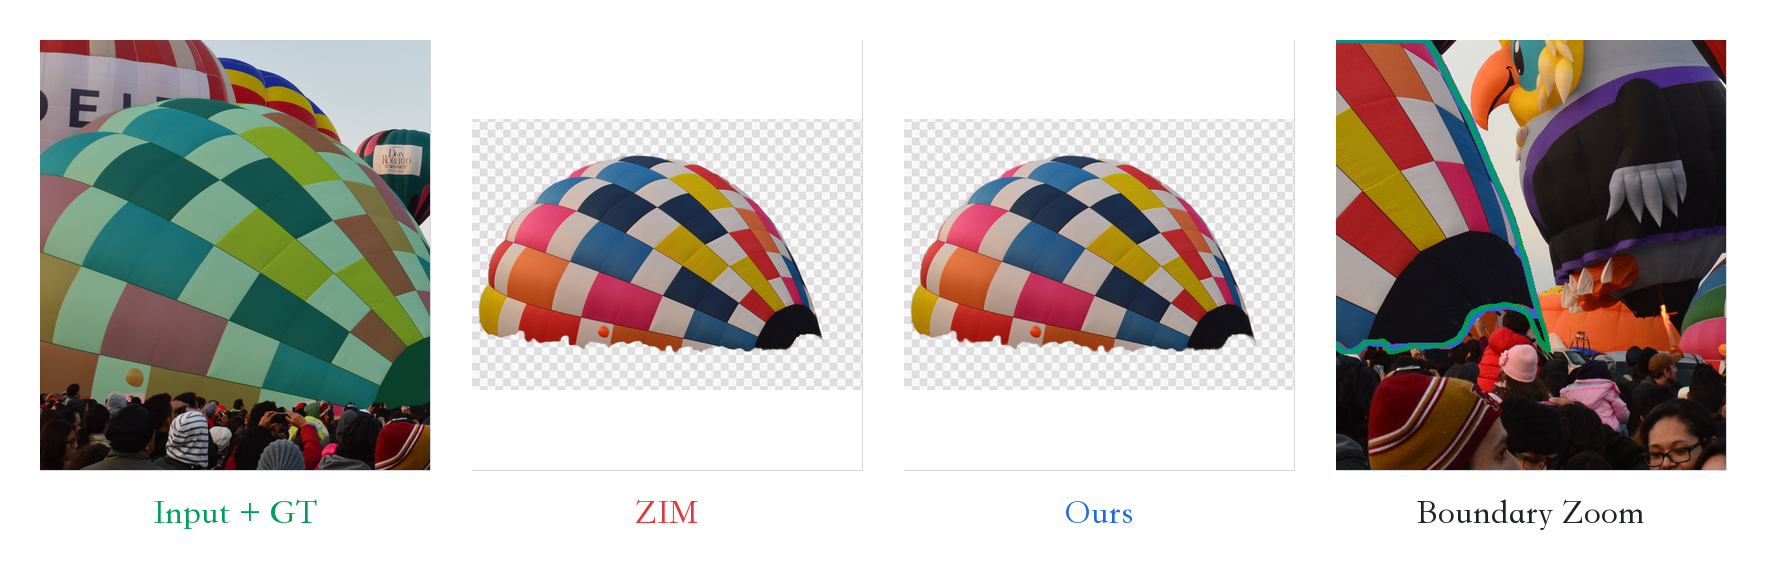
\includegraphics[width=0.32\linewidth]{zim_balloon.png}}
\caption{精细抠图定性对比（红：ZIM 基线，绿：GT，蓝：本文）。
无论大目标、细结构还是复杂弧形边界，本文边界都更贴近真值。}
\label{fig:zim_cases}
\end{figure*}

从三个案例的对比可以看到，本文方法的增益主要集中在边界区域——这与主表中
Boundary SAD 相对基线下降 $13.35\%$ 的提升最为突出相一致，也印证了
“注入边界一致性先验”的设计动机：在硬边、斜边与弧形边界上，蓝色轮廓都更贴近绿色的 GT，
换背景后不易出现白边、黑边或背景漏入。

\subsection{视频时序平滑}
\label{sec:exp-video}
\tabref{tab:video} 比较 7 种时序平滑策略。
Median 的 TC 提升最大，但 SAD/MSE 恶化严重、发丝模糊不可接受；
而\textbf{双向时序平滑（Bidirectional）}是唯一能在\emph{几乎不损精度}
（SAD 仅 $+0.44\%$，MSE 甚至 $-0.12\%$）的前提下提升 TC 的策略，细节保留最佳。
\figref{fig:video} 的散点图、雷达图与排名进一步说明：Bidirectional 最接近“TC 升、误差降”的理想区域，
综合最均衡，因此作为默认策略（$\alpha=0.7$）。
若追求更大的 TC 提升而能容忍轻微精度损失，Gaussian（$\sigma=2.0$、窗口 $=5$）是一个平衡选择，
其 TC 提升约 $4.0\%$、SAD 仅增加约 $2.4\%$。\figref{fig:gauss} 的参数敏感性分析显示：
增大 $\sigma$ 会同时抬高 TC 与 SAD（气泡越大表示 TC 提升越多、颜色越暖表示 SAD 恶化越重），
而窗口超过一定大小后收益饱和——这进一步支持了 $\sigma=2.0$、窗口 $=5$ 的折中取值。
整体而言，只在边界带上施加时序平滑，是“稳定时序”与“保住细节”之间的关键折中。

\begin{figure}[t]
\centering
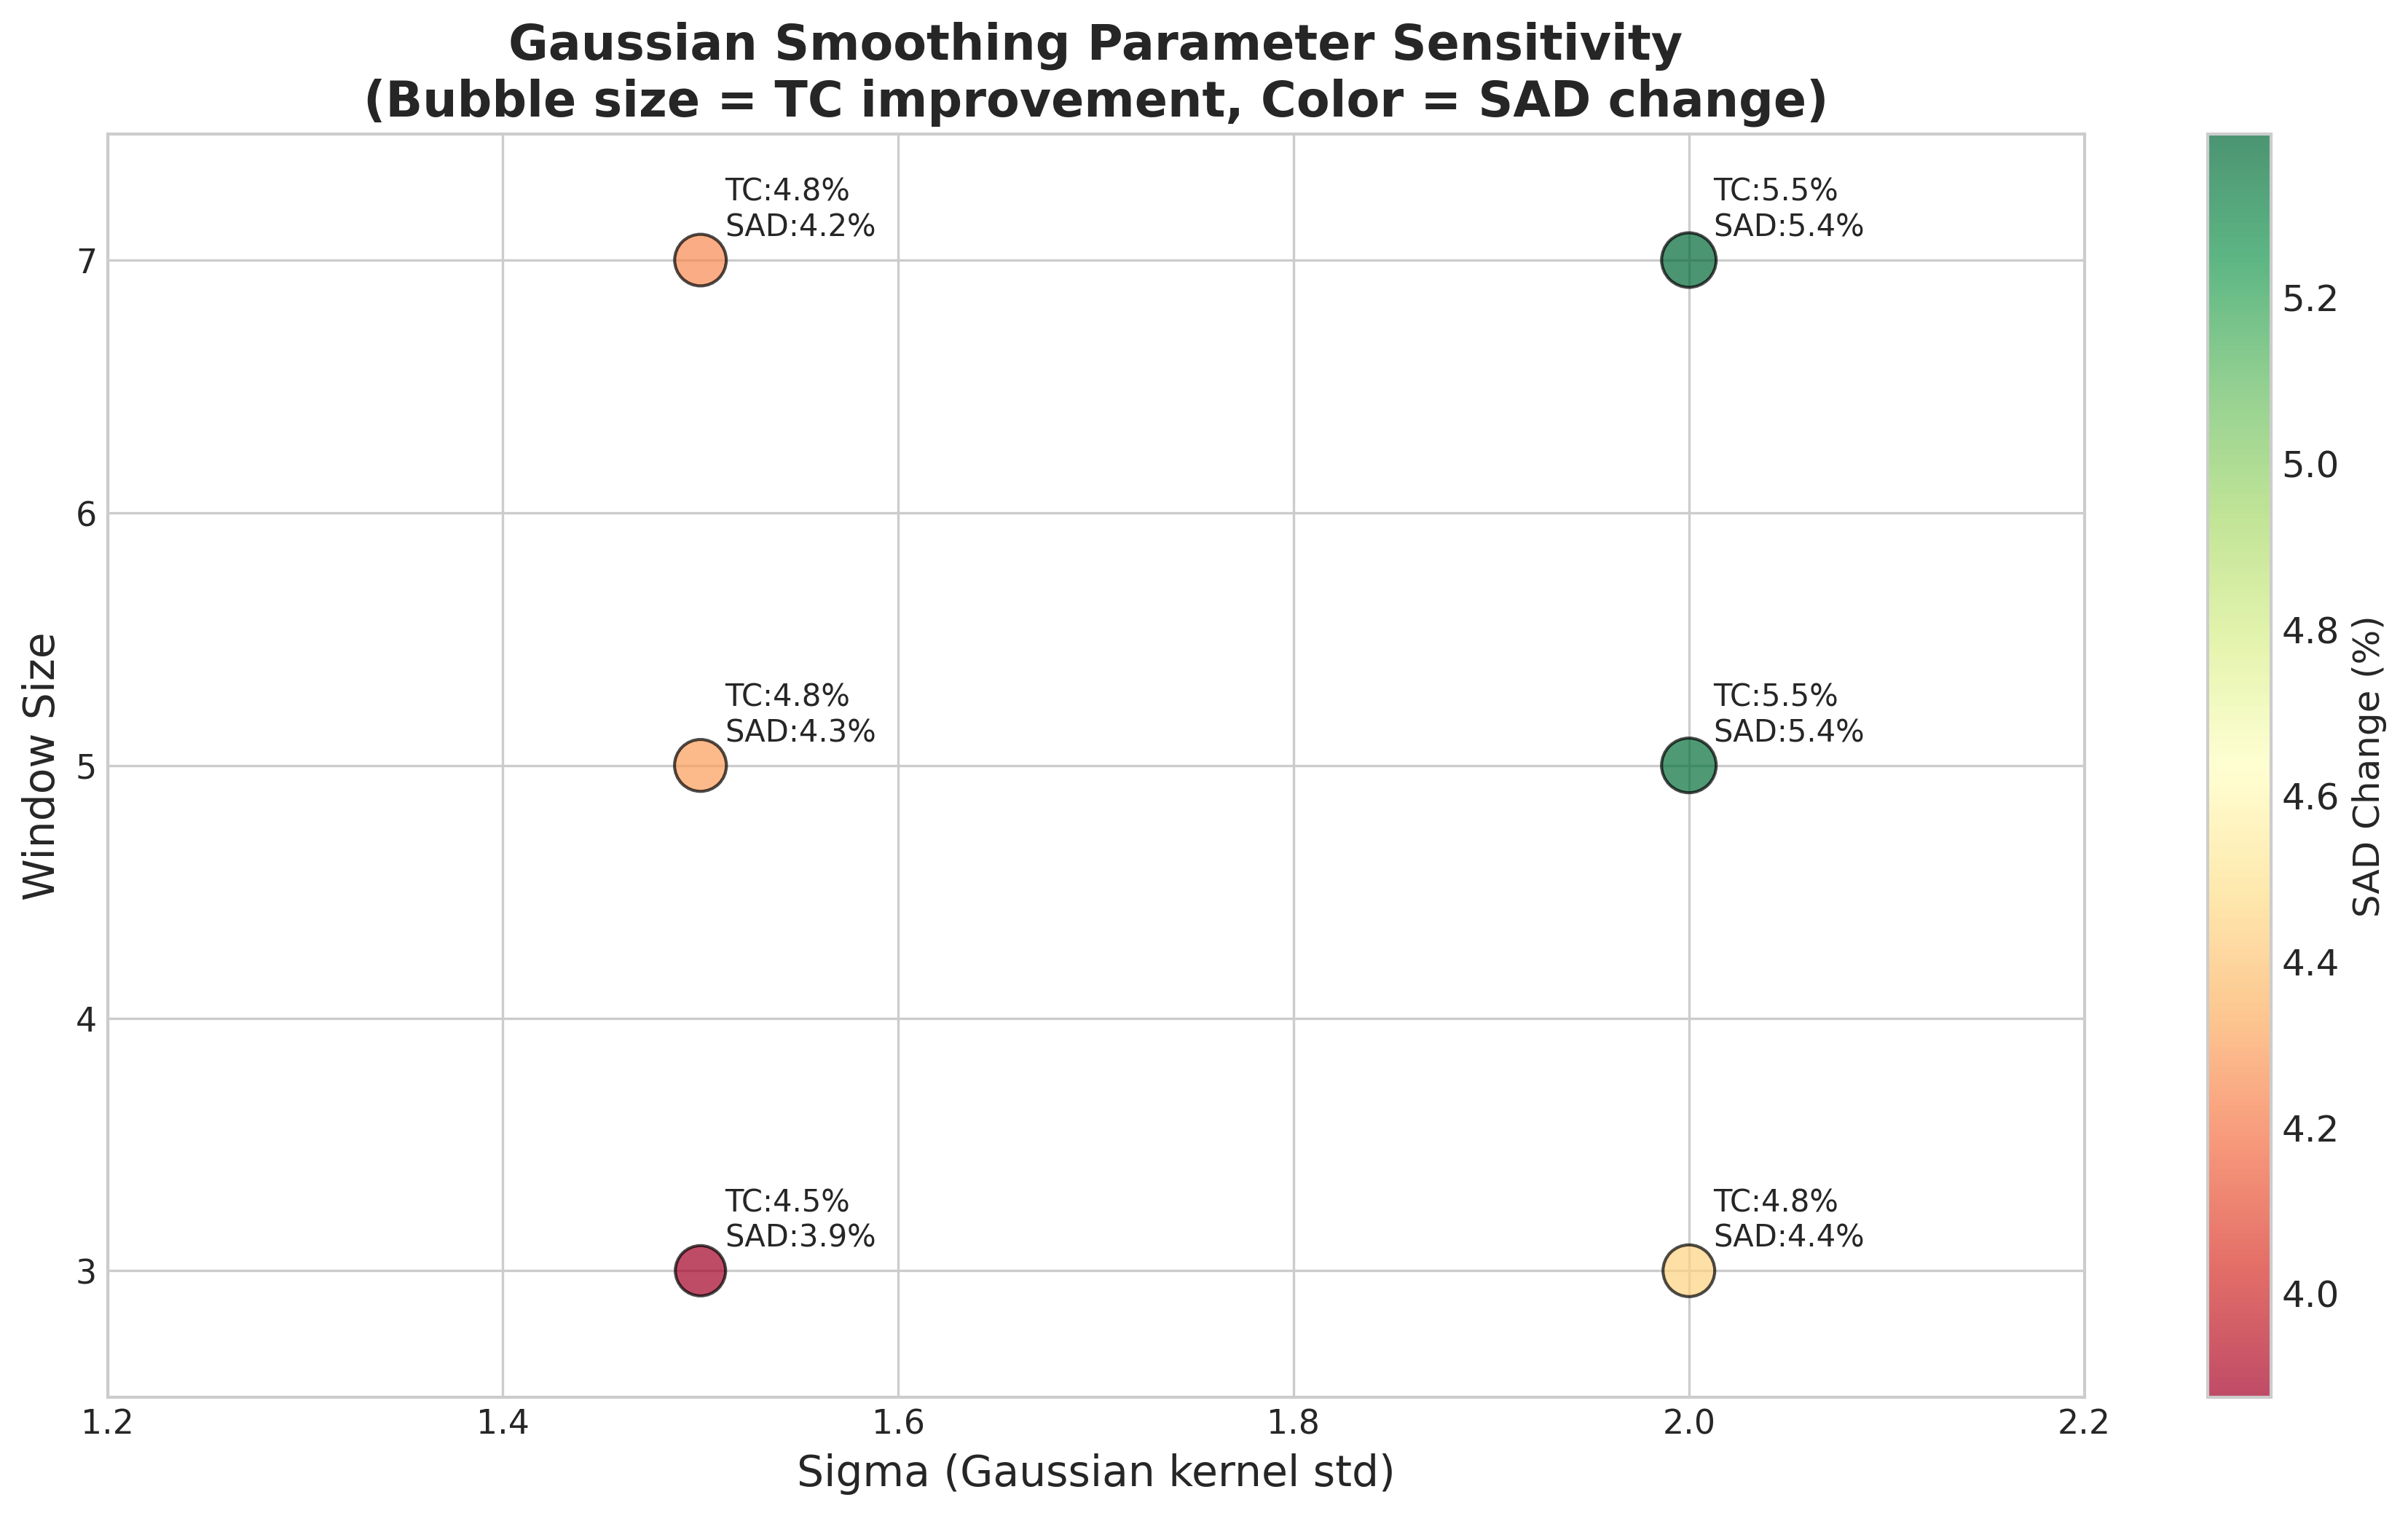
\includegraphics[width=0.86\linewidth]{vid_gaussian.png}
\caption{Gaussian 时序平滑的参数敏感性：气泡大小表示 TC 提升、颜色表示 SAD 变化。
增大 $\sigma$ 提升 TC 但恶化 SAD，窗口增大后收益饱和。}
\label{fig:gauss}
\end{figure}

\noindent\textbf{跨数据集稳定性。}在 YouTubeMatte 与更具挑战性的 VideoMatt 两个数据集上，
各方法在前者普遍表现更好；VideoMatt 含更多复杂运动与精细结构，平滑难度更高。
箱线图（见附录）显示 Bidirectional 的 SAD 变化分布最集中、异常值最少，
说明其精度在不同视频间最稳定、跨场景泛化最好，因而适合作为默认策略。

\begin{table}[t]
\centering
\small
\setlength{\tabcolsep}{4pt}
\begin{tabular}{lrrrl}
\toprule
方法 & TC 提升 & SAD 变化 & MSE 变化 & 细节 \\
\midrule
Median & 6.68\% & $+8.88\%$ & $+23.91\%$ & Poor \\
Gaussian & 4.00\% & $+2.40\%$ & $+3.00\%$ & Fair \\
Adaptive & 3.62\% & $+3.12\%$ & $+5.88\%$ & Fair \\
Guided EMA & 3.49\% & $+2.99\%$ & $+5.28\%$ & Fair \\
\textbf{Bidirectional} & \textbf{2.89\%} & \textbf{$+0.44\%$} & \textbf{$-0.12\%$} & \textbf{Excellent} \\
EMA & 2.59\% & $+1.64\%$ & $+2.40\%$ & Good \\
Flow & 1.55\% & $+2.15\%$ & $+3.62\%$ & Fair \\
\bottomrule
\end{tabular}
\caption{20 段视频上的 7 种时序平滑策略对比。Bidirectional 精度几乎无损且细节最佳。}
\label{tab:video}
\end{table}

\begin{figure}[t]
\centering
\subfigure[TC--SAD 散点]{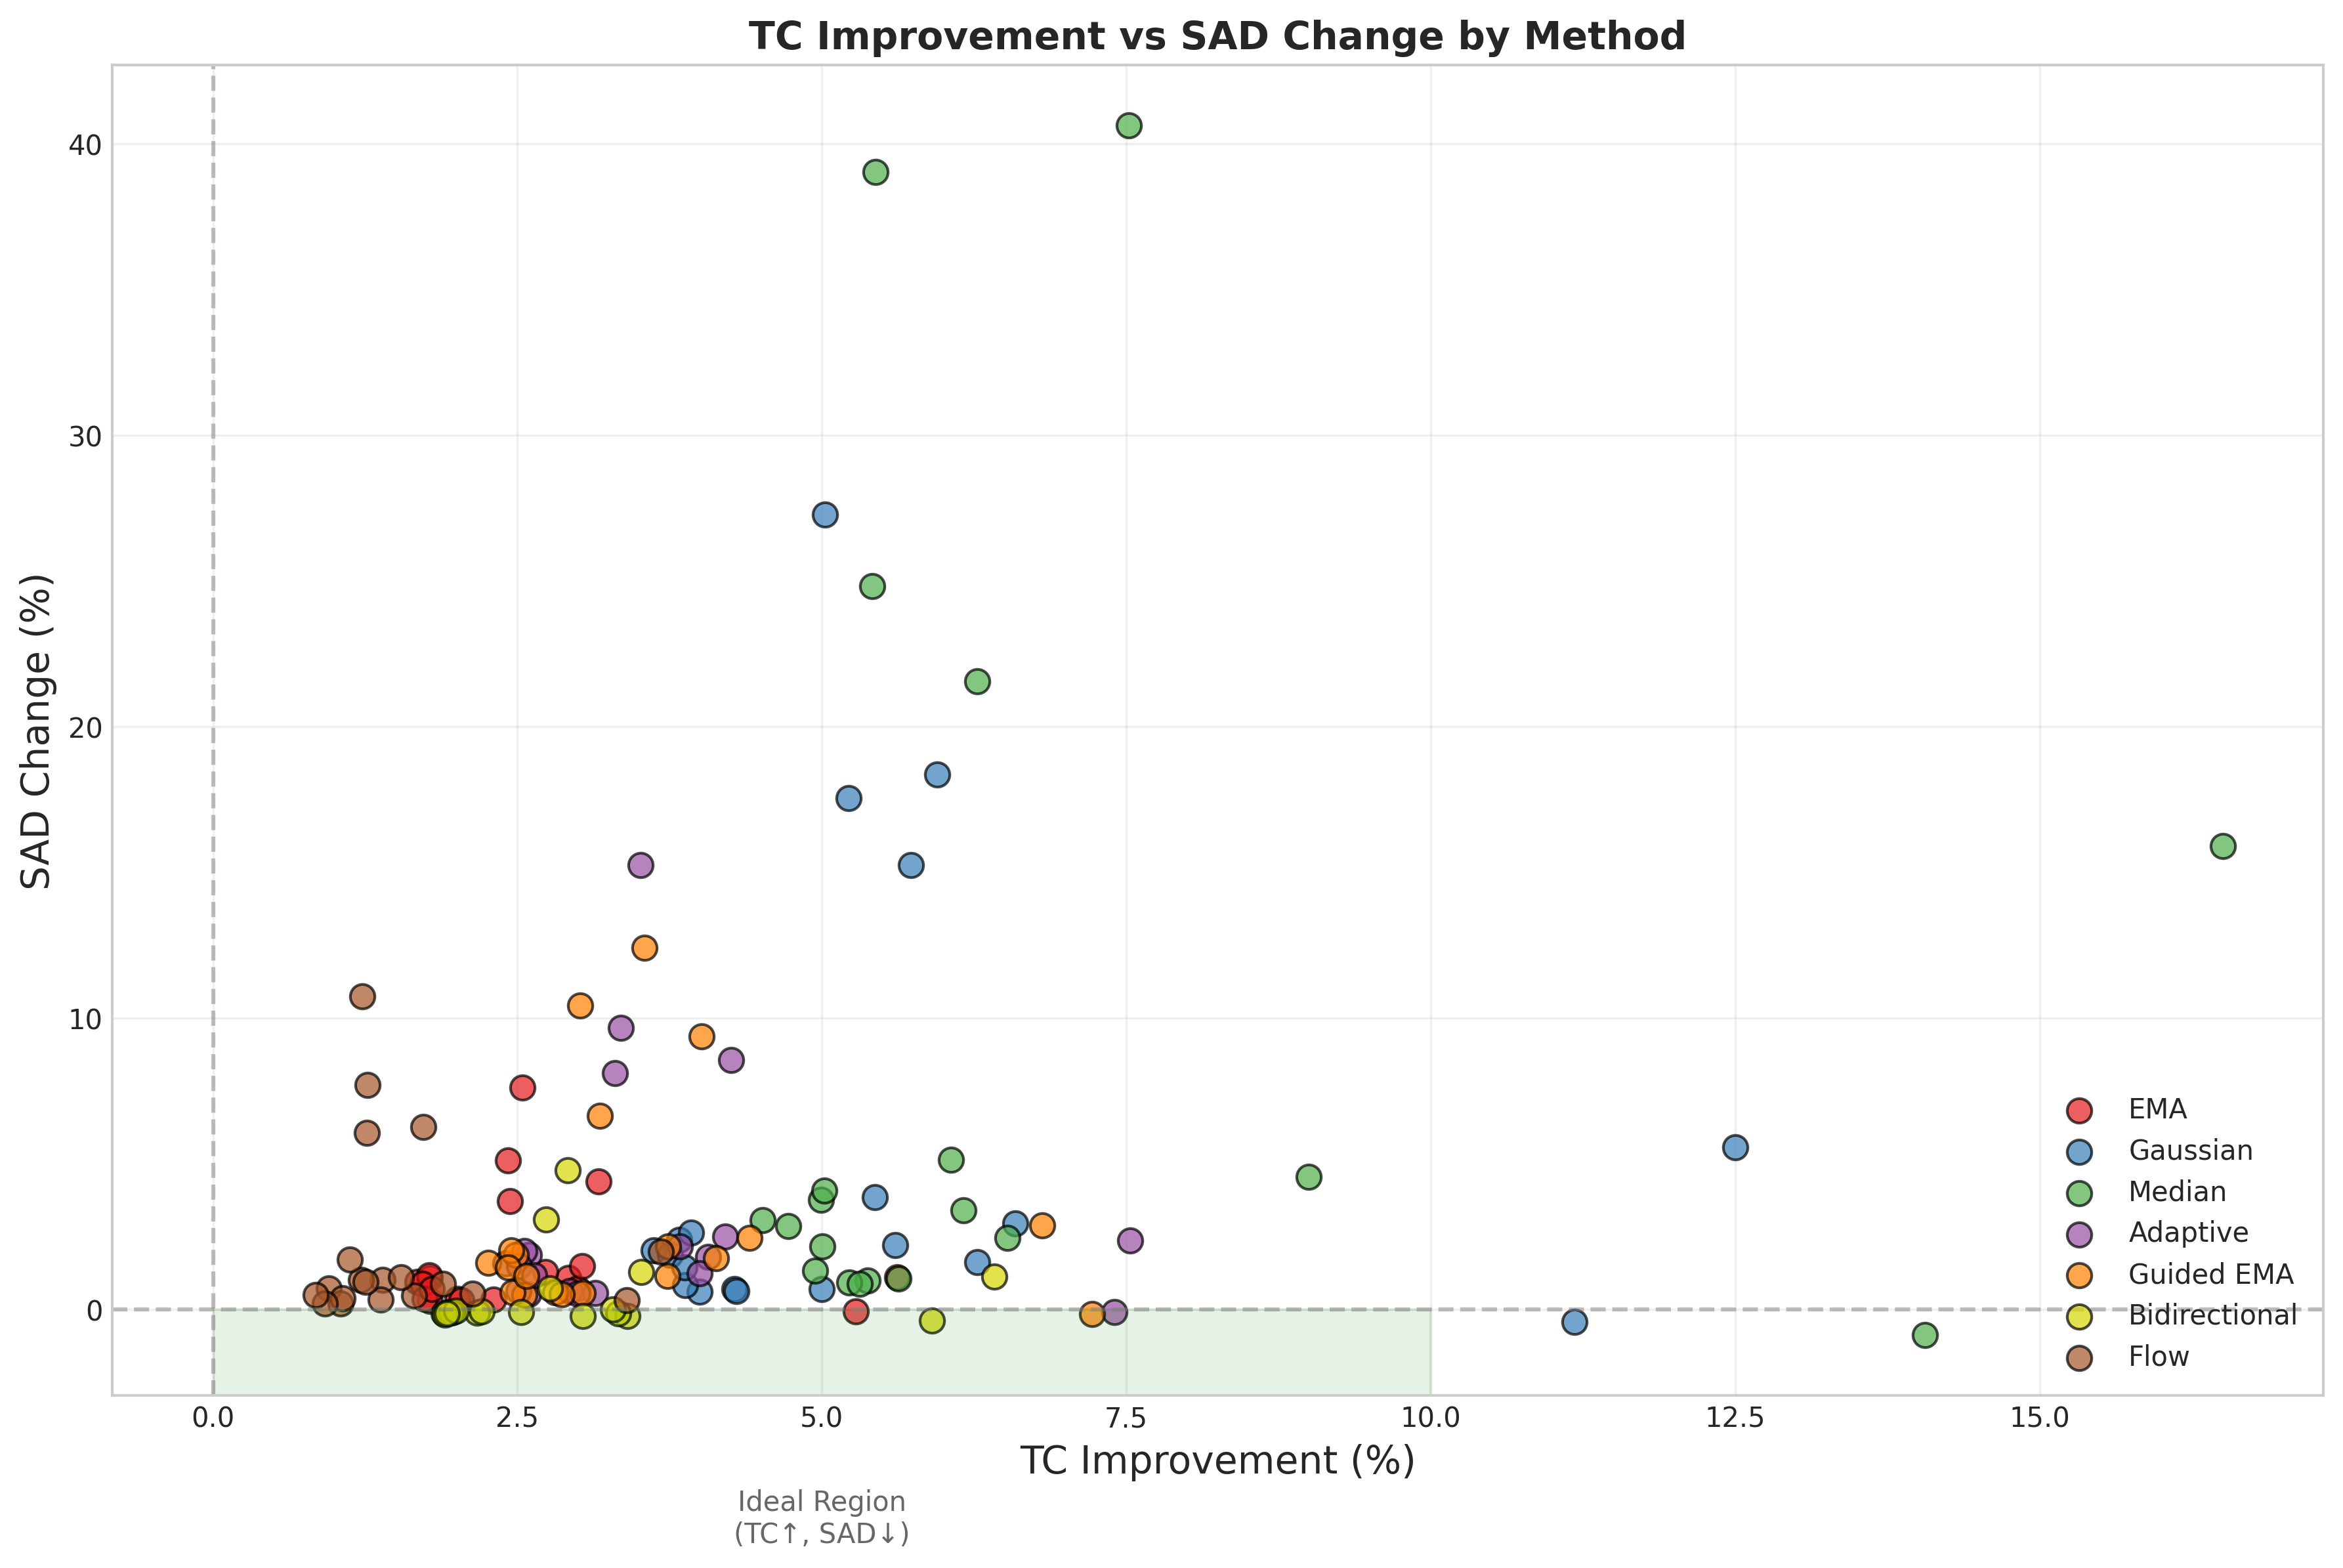
\includegraphics[width=0.48\linewidth]{vid_scatter.png}}
\subfigure[综合雷达图]{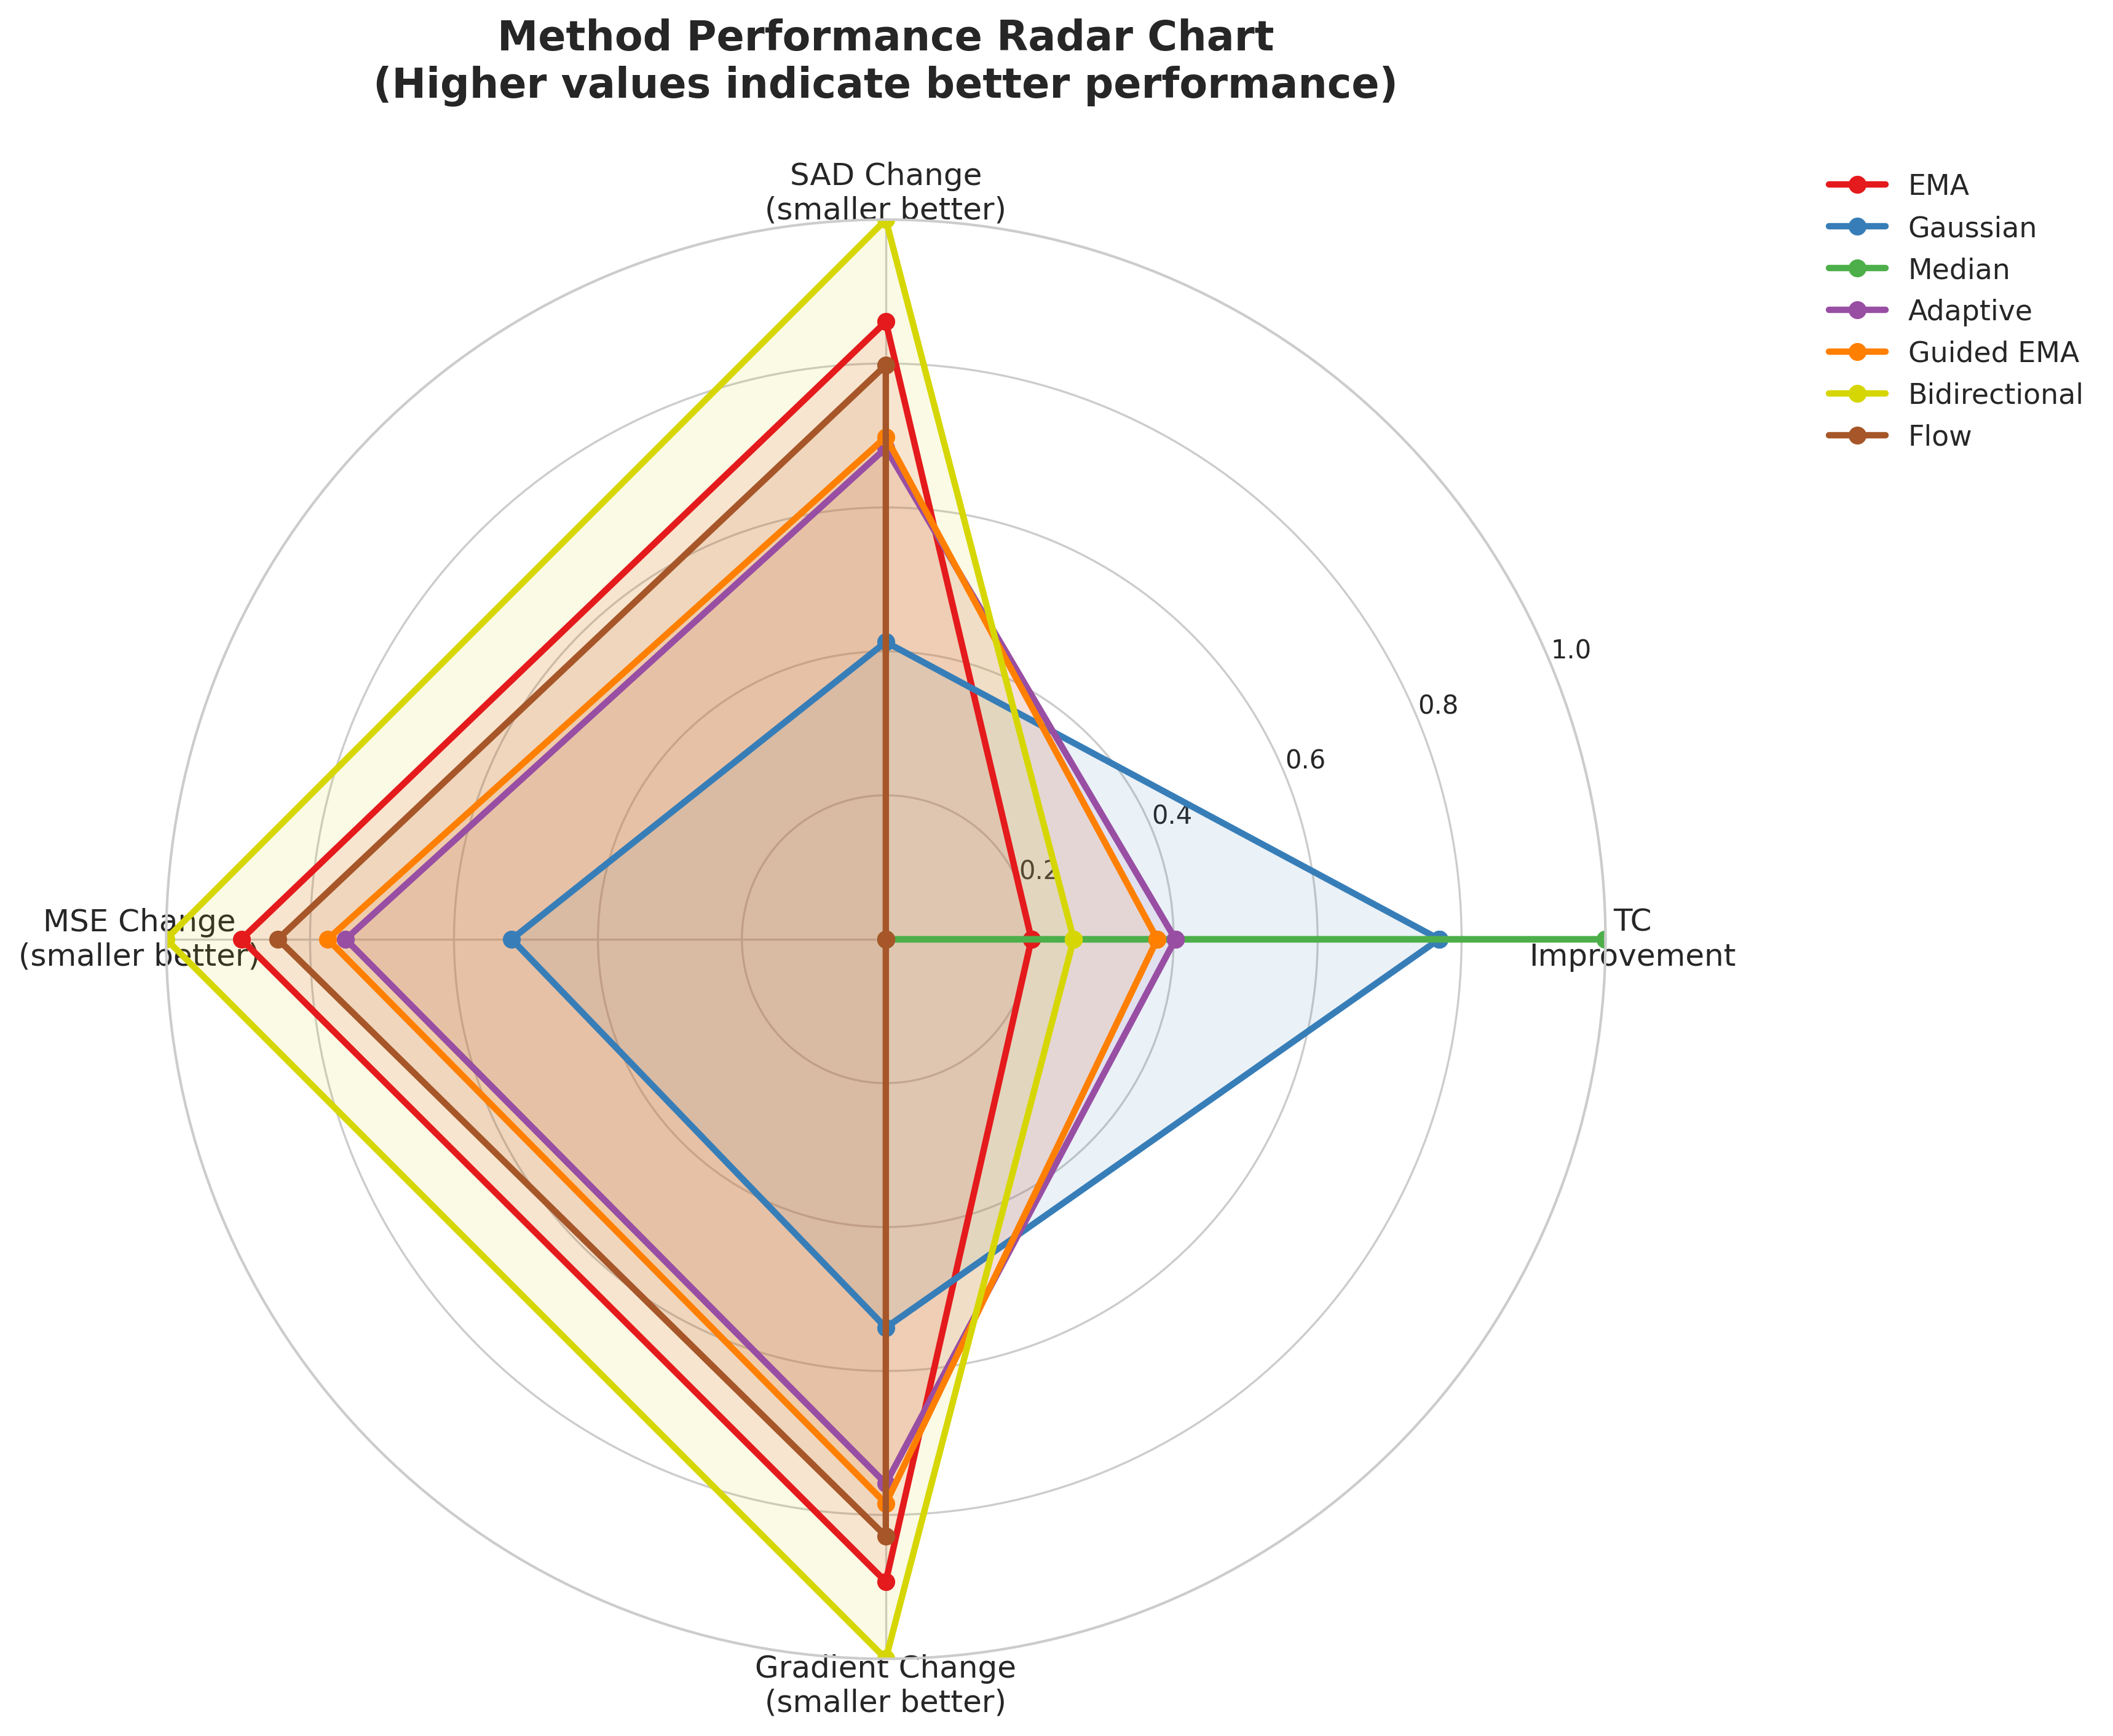
\includegraphics[width=0.48\linewidth]{vid_radar.png}}
\caption{视频时序平滑分析。Bidirectional 最接近理想区域、综合最均衡。}
\label{fig:video}
\end{figure}

\subsection{应用：RGBA 与 Composer}
\label{sec:exp-app}
我们将优化后的 $\alpha$ 作为 RGBA 的透明通道，得到透明前景，并据
\equref{eq:matting} 完成换背景与背景虚化。该模块不重新预测目标、不计入 valid706，
仅用于检验 $\alpha$ 接入真实编辑流程后的边界质量。
\figref{fig:composer} 显示，换背景与虚化后主体边缘仍贴合紧密，无明显白边、黑边或空洞，
说明边界优化不仅体现在指标上，落到最终编辑同样干净。

\begin{figure}[t]
\centering
\subfigure[整车]{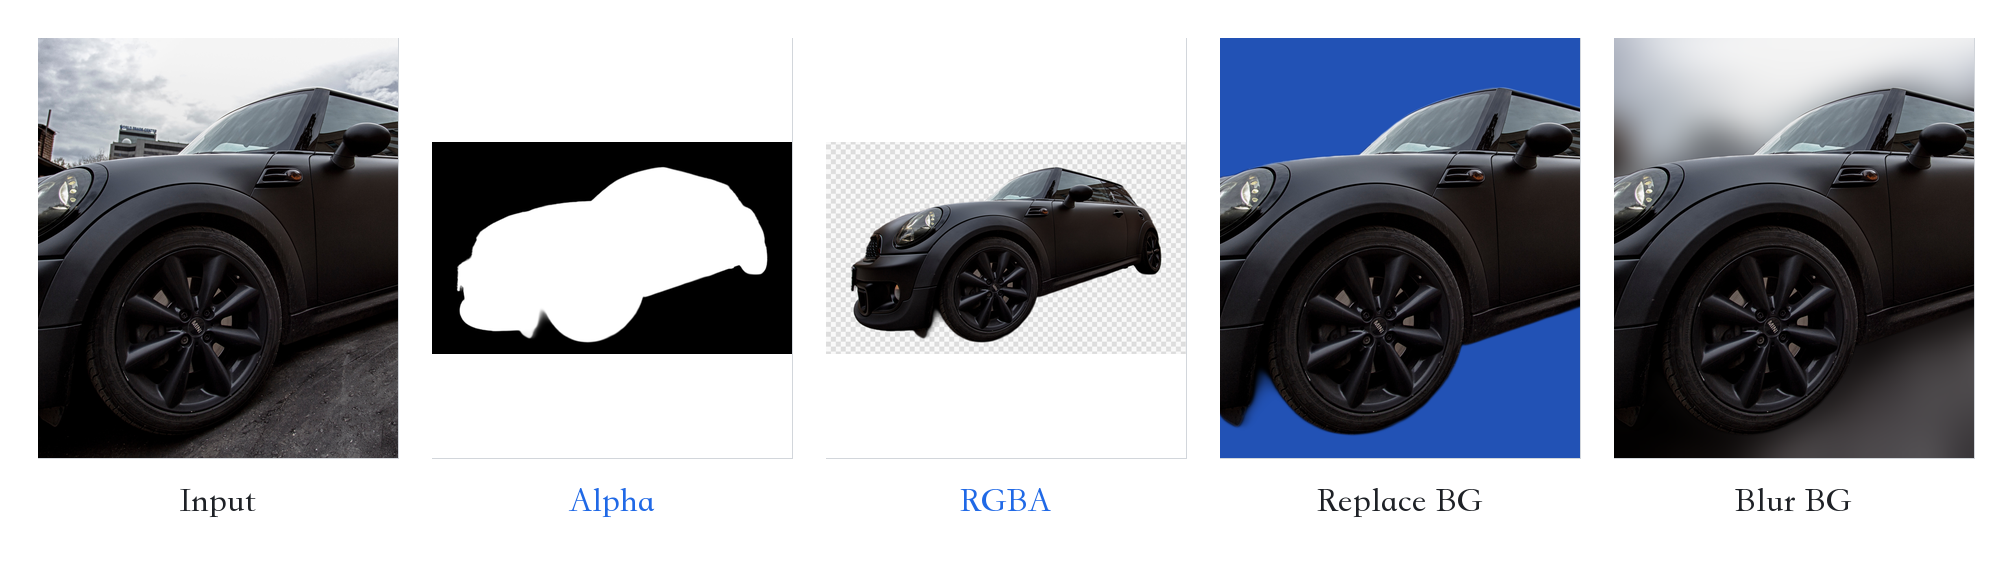
\includegraphics[width=0.48\linewidth]{composer_car.png}}
\subfigure[设备部件]{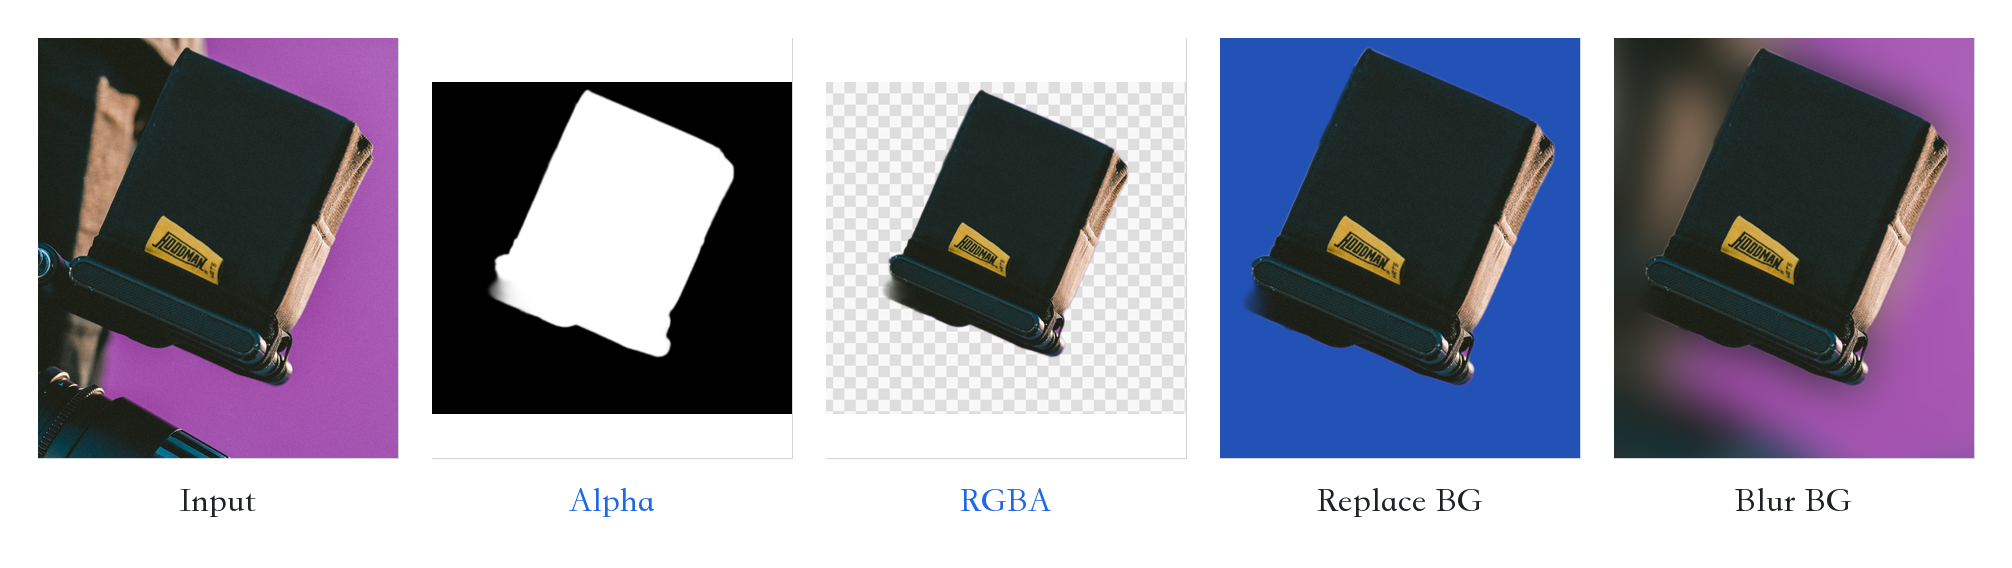
\includegraphics[width=0.48\linewidth]{composer_device.png}}
\caption{Composer 应用：RGBA 前景、背景替换与背景虚化的轮廓基本一致，边界干净。}
\label{fig:composer}
\end{figure}

\section{讨论与局限}
\label{sec:discussion}
本文方法以零训练换取了强可复现性与模块解耦，但也带来若干内在局限。
其一，性能上界受基础模型制约：抠图质量本质上由 ZIM 的预测能力决定，
我们的先验只能在其输出上做无训练的细化，无法弥补基础模型在极端材质（如大面积透明体）上的系统性偏差。
其二，对提示质量有依赖：上游若给出明显偏移的 bbox，BSP 的“目标必在框内”假设会失效，
甚至可能压制到真实前景；我们用框的轻微外扩与边缘模糊来缓解，但并不能完全消除。
其三，推理开销：翻转 TTA 使前向次数翻倍，多尺度推理进一步带来约三倍开销，
在对延迟敏感的场景需要权衡。其四，视频端 TC 与精度之间存在折中，
双向平滑选择了“精度近乎无损”的一端，若场景更看重时序稳定，则需要切换到更激进的策略。
这些局限也指出了后续改进的方向。

\section{结论}
\label{sec:conclusion}
本文提出零训练的精细抠图与换背景系统 PromptMatte，将 SAM2 定位、ZIM 精细抠图、
视频时序稳定与背景编辑统一为一条主线。其核心是一条\textbf{一致性先验}：
它在图像上以 PromptMatte-TTA-GF（翻转等变）与 BSP（空间先验）的形式注入 ZIM 输出，
在视频上复用为双向时序平滑（时序一致），并通过首帧复用把图像与视频接成同一套方法。
实验表明，本文方法在 valid706 上四项指标全面优于 ZIM 基线，在视频上以几乎无损精度的代价
提升时序一致性。未来工作包括把一致性先验进一步统一为可学习的轻量正则，
以及在更大规模数据上验证。

\noindent\textbf{分工。}史傅冠华负责上游开放词汇分割（\secref{sec:upstream}）；
梁景铭负责精细抠图与系统整合（\secref{sec:matting}）；
张竣翔负责视频时序平滑（\secref{sec:video}）。

{\small
\bibliographystyle{ieee}
\begin{thebibliography}{99}
\bibitem{sam} A.~Kirillov \etal. Segment Anything. In \emph{ICCV}, 2023.
\bibitem{sam2} N.~Ravi \etal. SAM 2: Segment Anything in Images and Videos. In \emph{ICLR}, 2025.
\bibitem{groundedsam} T.~Ren \etal. Grounded SAM: Assembling Open-World Models for Diverse Visual Tasks. arXiv:2401.14159, 2024.
\bibitem{zim} B.~Kim \etal. ZIM: Zero-Shot Image Matting for Anything. In \emph{ICCV}, 2025.
\bibitem{mam} J.~Li, J.~Jain, and H.~Shi. Matting Anything. In \emph{CVPR}, 2024.
\bibitem{matanyone} P.~Yang \etal. MatAnyone 2: Scaling Video Matting via a Learned Quality Evaluator. arXiv, 2026.
\bibitem{gf} K.~He, J.~Sun, and X.~Tang. Guided Image Filtering. In \emph{ECCV}, 2010; \emph{IEEE TPAMI}, 2013.
\end{thebibliography}
}

\clearpage
\appendix
\section{附录}

\subsection{完整消融与实现细节}
\label{sec:appendix-impl}
\noindent\textbf{上游分割。}\tabref{tab:sam} 已给出 8 种组合的完整消融。
模型为 SAM2.1 Hiera-Base+（80.8M 参数），A10 上约 $1.16$ it/s（bbox-only）。
重排序权重见 \equref{eq:rerank}；多尺度取 $\{0.75,1.0,1.25\}\times$。

\noindent\textbf{精细抠图。}ZIM ViT-B，official bbox 提示。
PromptMatte-TTA-GF 见 \equref{eq:ttagf}：水平翻转 TTA + 半径为 1 的 Guided Filter；
BSP 见 \equref{eq:bsp}：框外保守抑制，对框做轻微外扩与边缘模糊以保护框边前景。
全过程冻结 ZIM、零训练。valid706 主表见 \tabref{tab:zim}。

\noindent\textbf{视频。}MatAnyone2 逐帧推理为基线，复用图像主线首帧 $\alpha$ 作为种子；
双向时序平滑仅作用于 $\alpha\in[0.05,0.95]$ 的边界带，$\alpha=0.7$。
7 种策略完整对比见 \tabref{tab:video}。

\subsection{更多可视化}
\label{sec:appendix-vis}
\figref{fig:appendix-vid} 给出视频时序平滑的补充分析与逐帧示例。
箱线图显示 Bidirectional 的 SAD 分布最集中、异常值最少，说明其精度在不同视频间最稳定；
两数据集对比显示其在 YouTubeMatte 与更具挑战性的 VideoMatt 上均表现稳健。

\begin{figure}[h]
\centering
\subfigure[各方法分布箱线图]{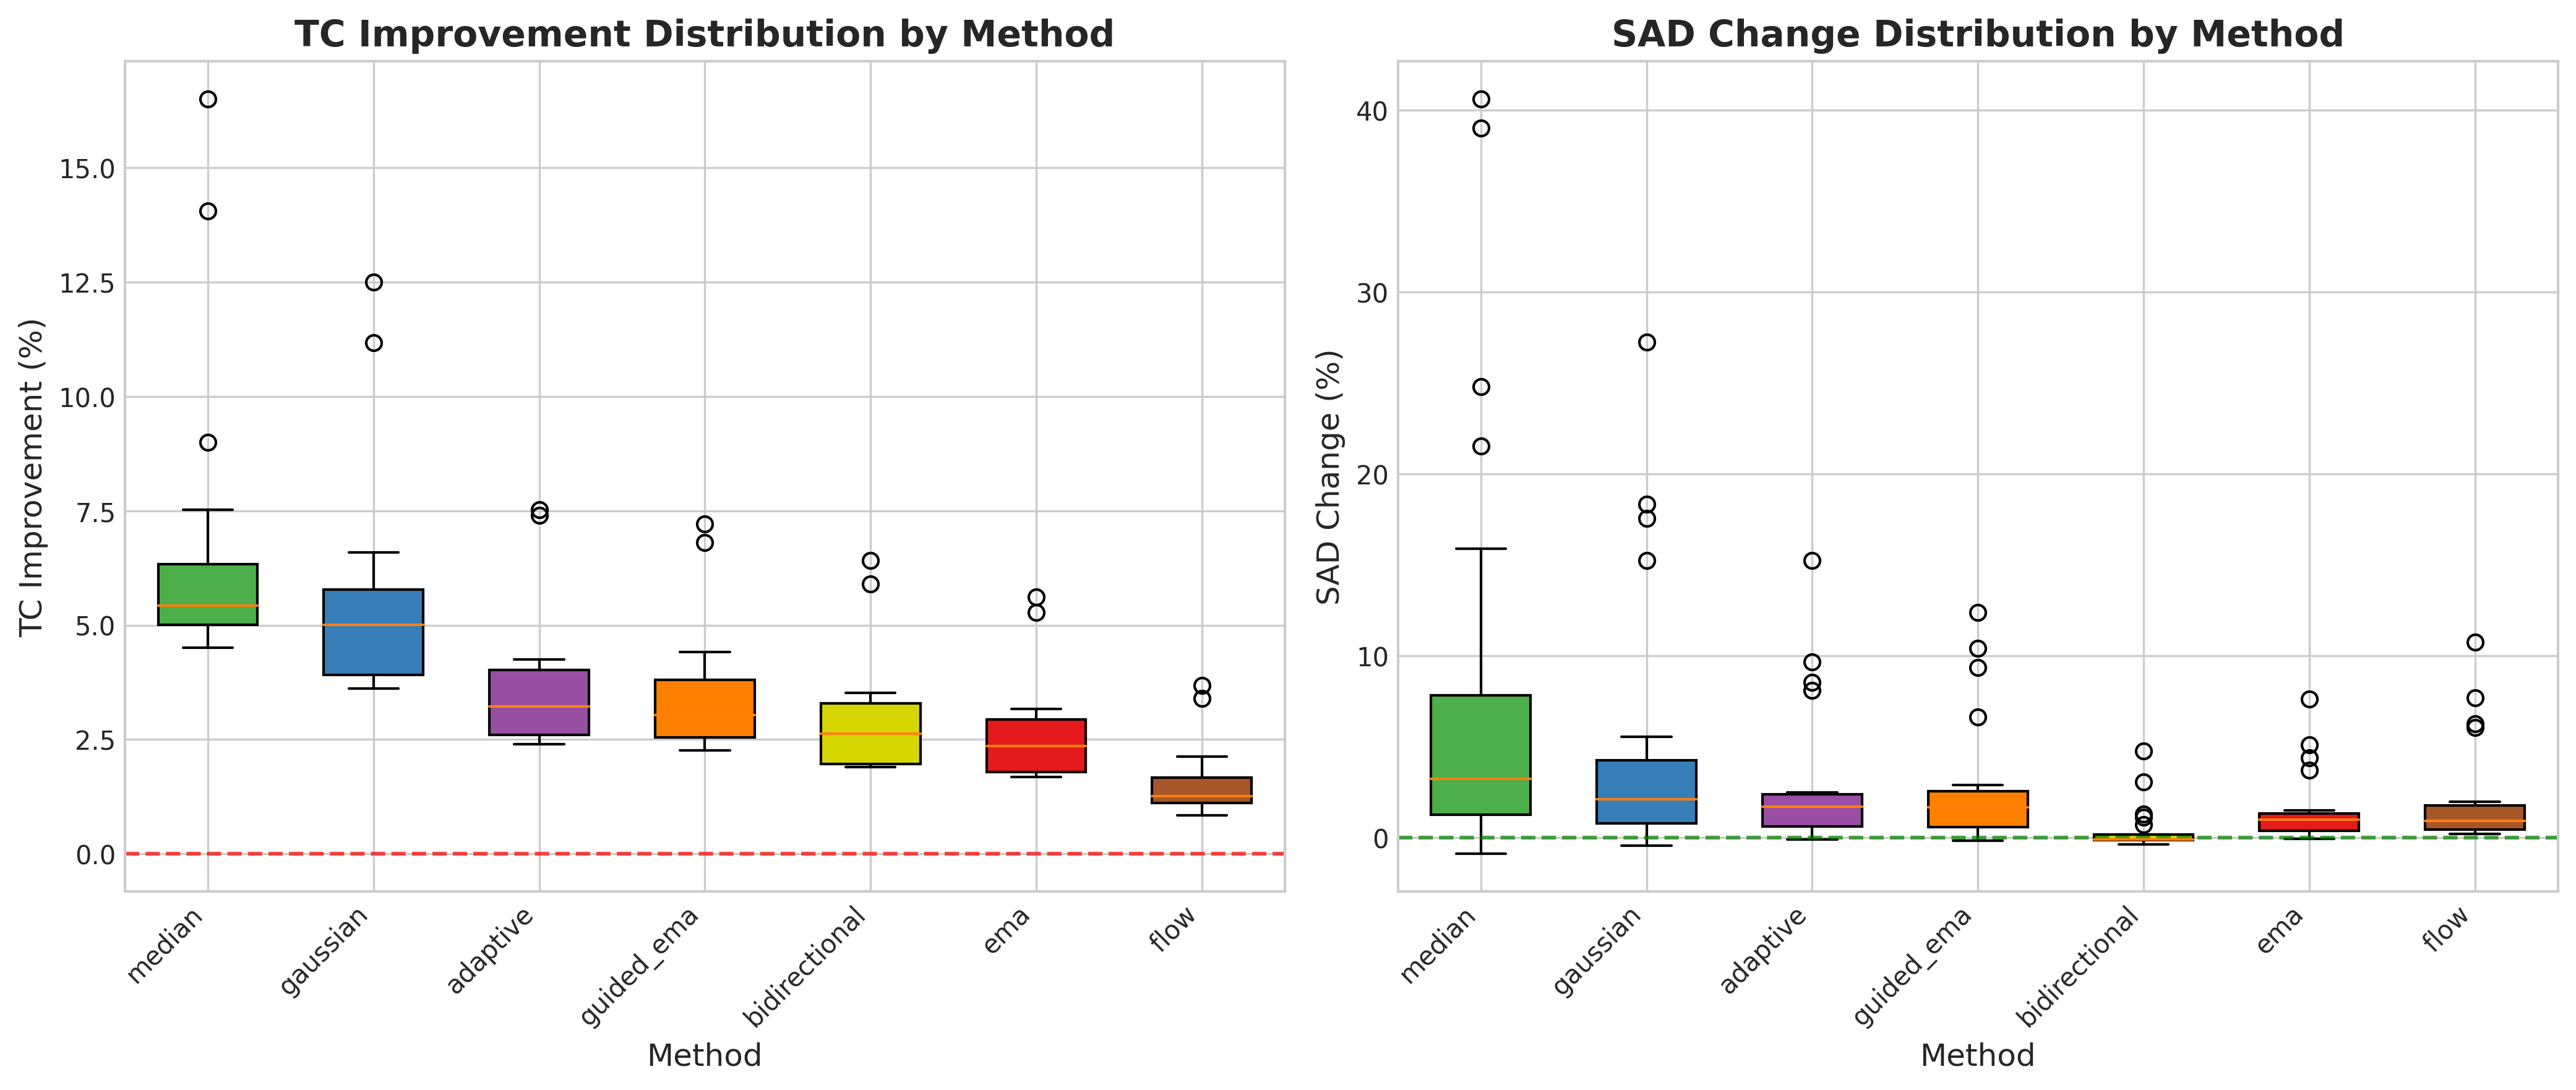
\includegraphics[width=0.48\linewidth]{vid_boxplot.png}}
\subfigure[两数据集对比]{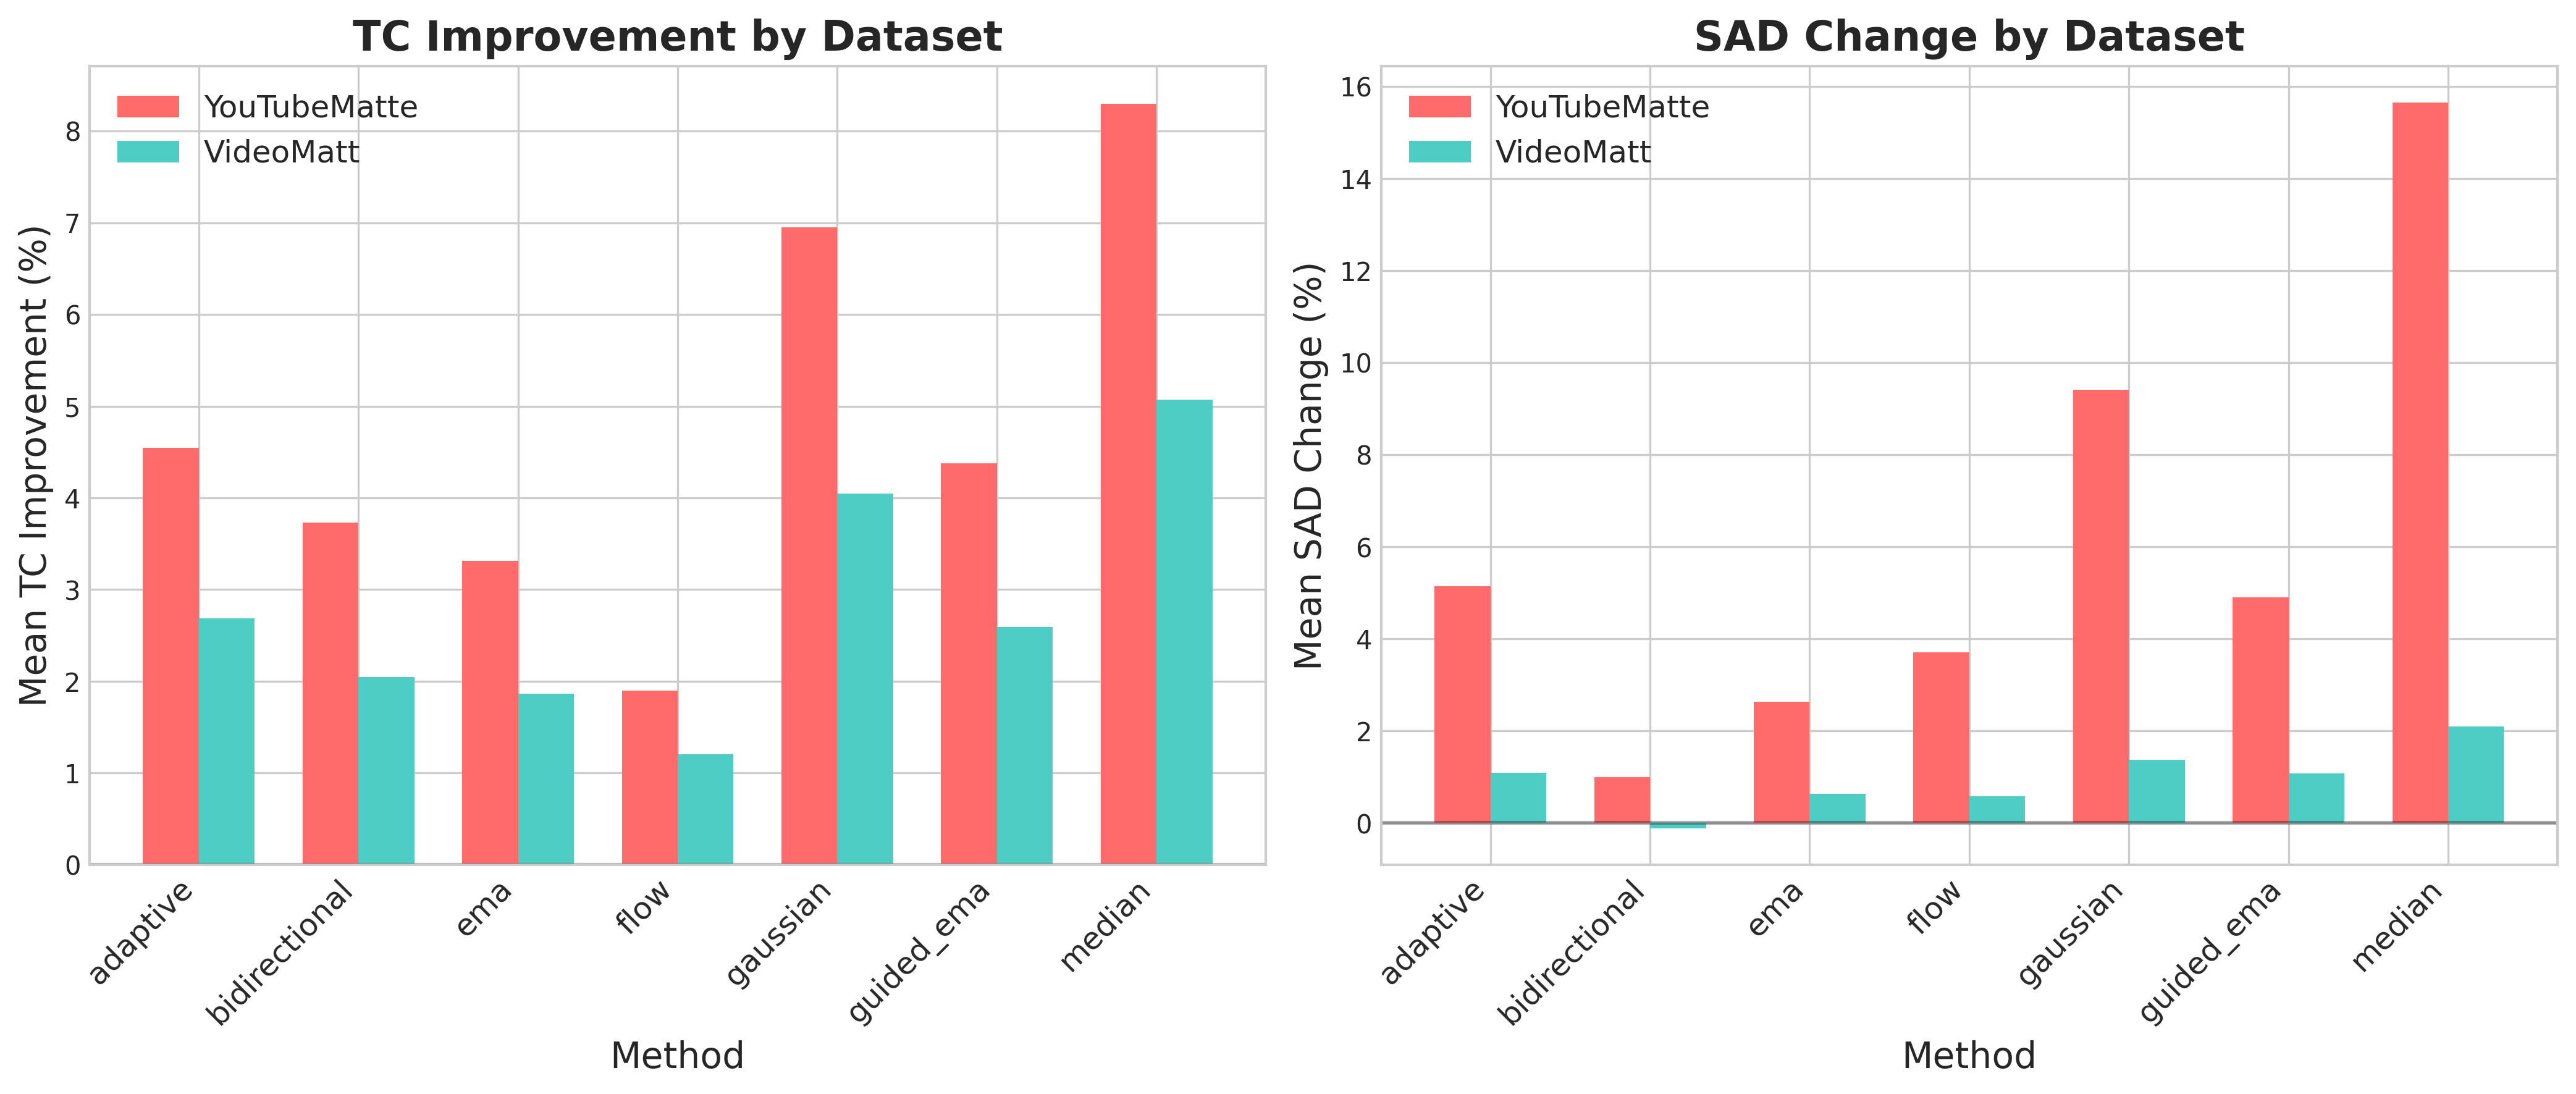
\includegraphics[width=0.48\linewidth]{vid_dataset.png}}\\
\subfigure[性能排名]{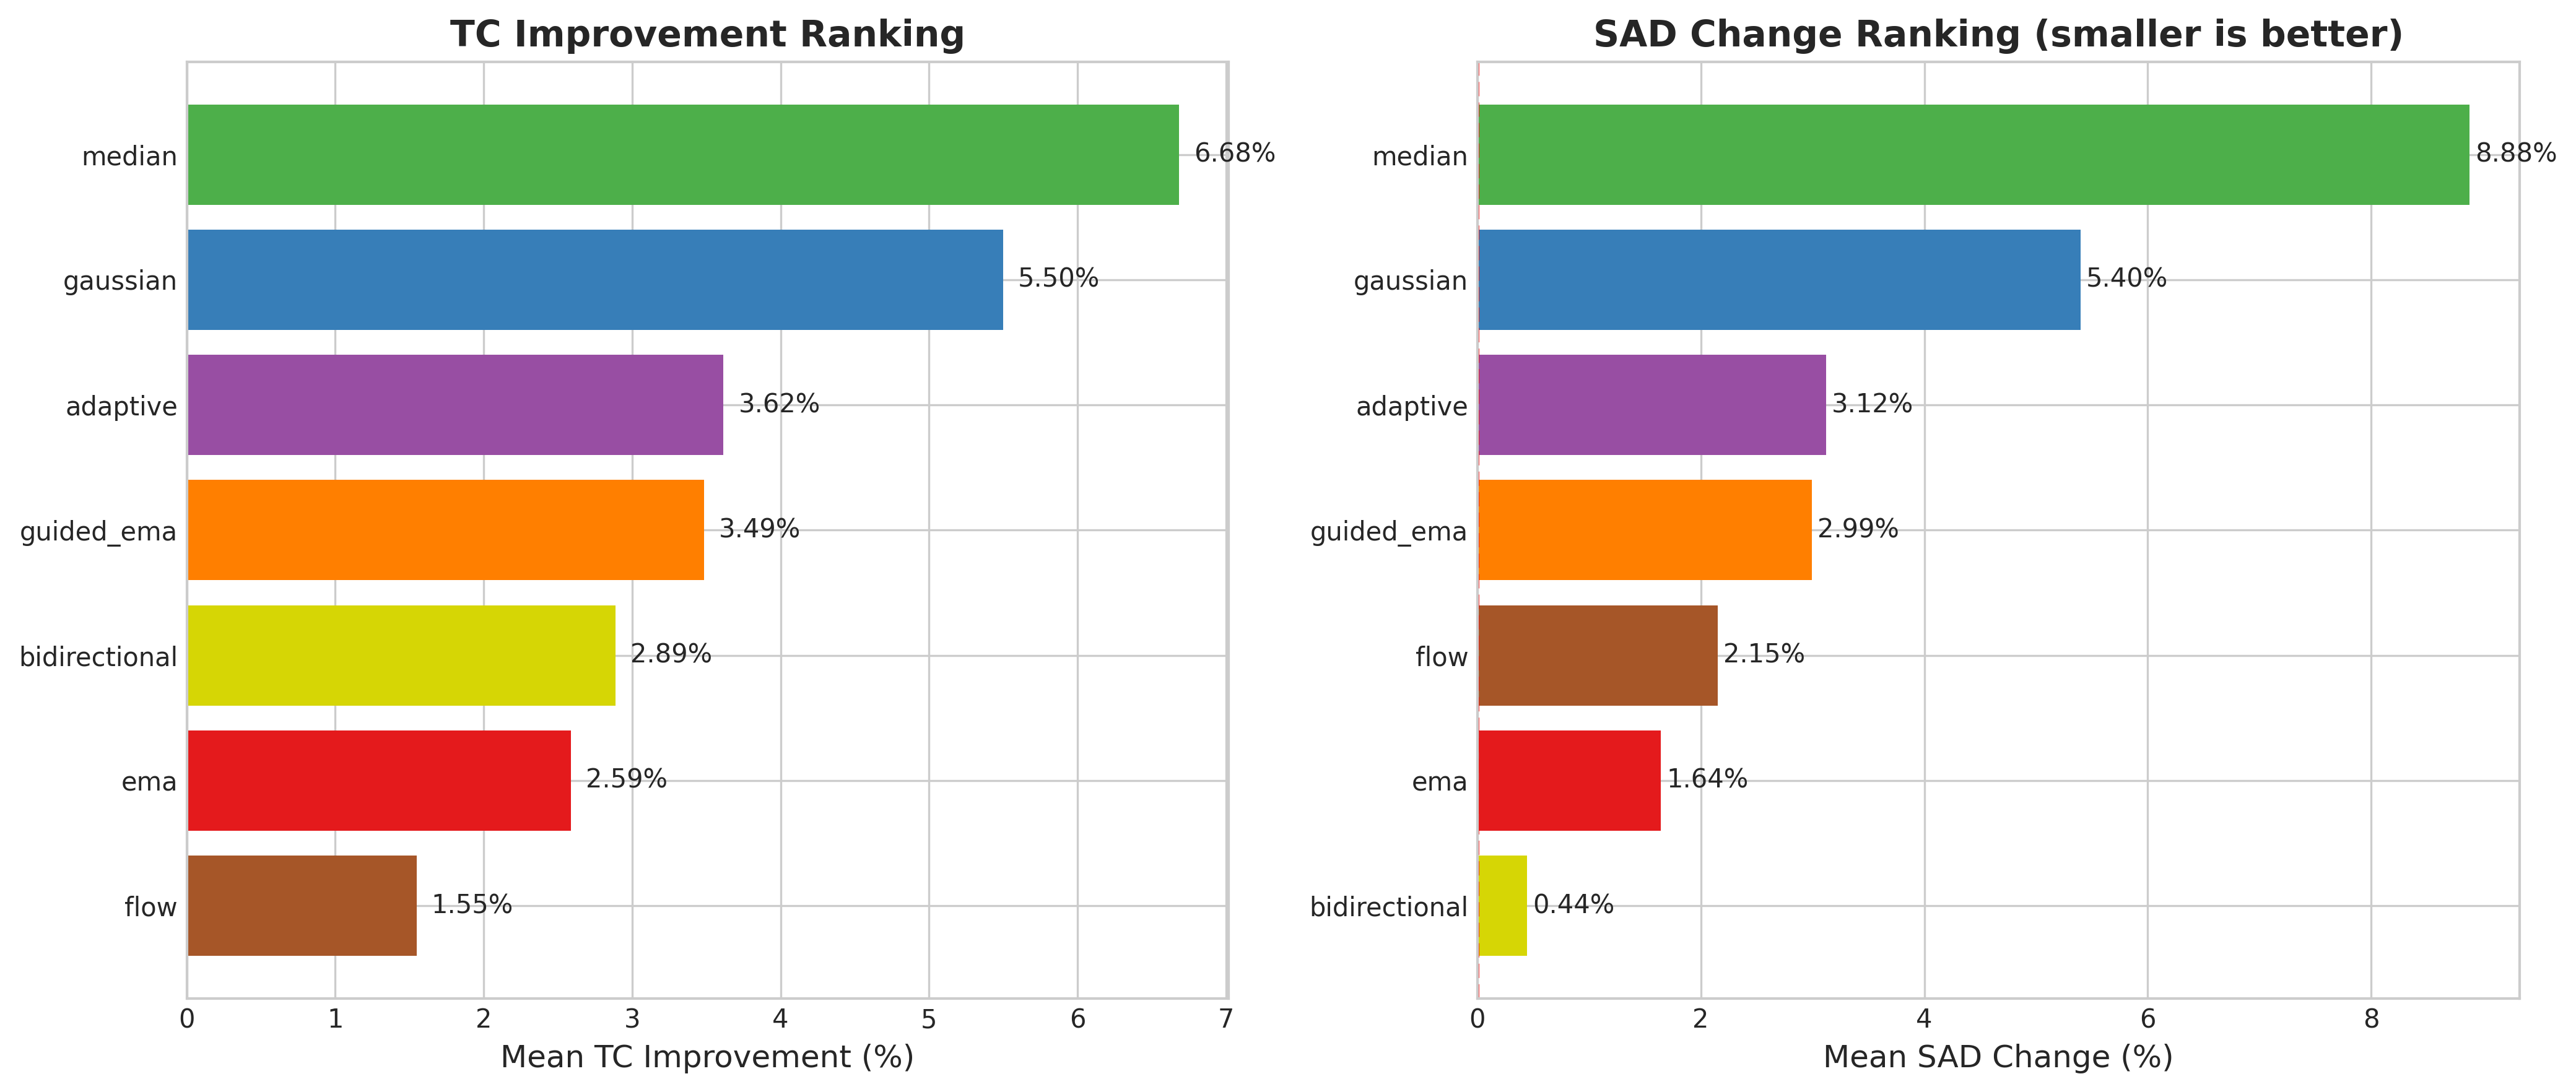
\includegraphics[width=0.48\linewidth]{vid_ranking.png}}
\subfigure[视频帧示例]{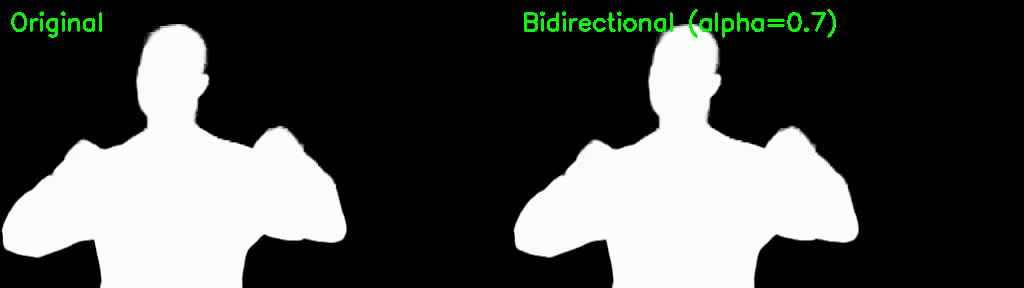
\includegraphics[width=0.48\linewidth]{vid_frame.png}}
\caption{视频时序平滑的补充可视化。}
\label{fig:appendix-vid}
\end{figure}

\end{document}
